\chapter{Aportaciones}

\section{Retropropagación en redes neuronales rotalmente conectadas}

En esta sección se analizará en profundidad el cálculo del gradiente de la pérdida respecto a cada parámetro entrenable de una red totalmente conectada, así como también respecto a la entrada y salida de cada capa. Primero se mostrarán los cálculos para unos ejemplos concretos, y una vez conocidas las bases sobre ellos, se mostrará cómo aplicarlos para cualquier tipo de red totalmente conectada. 

\subsection{Retropropagación en capa SoftMax, \cite{Cross_entropy_backprop} \cite{Cross_entropy_backprop_grad_input}} 

Tal y como se comentó en secciones anteriores, se empleará SoftMax en la última capa totalmente conectada. Así, se definen los valores de entrada a la misma como Z, y los de salida como O, tal y como se muestra en la Figura \ref{cross_entropy_notacion}.

\begin{figure}[H]
	\centering
	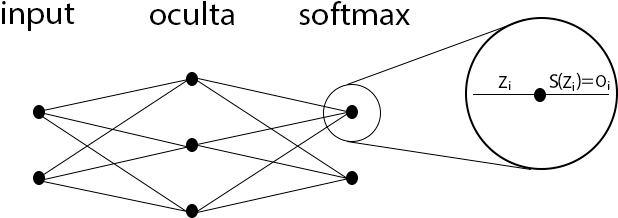
\includegraphics[scale=0.4]{imagenes/NN_softmax.jpg}  
	\caption{Estructura de una red totalmente conectada con softmax en la última capa}
\end{figure}

\begin{gather}
	E = - \sum_{i=1}^{H}  [y_i * log(O_i)] 
	\label{cross_entropy_notacion}
\end{gather}

Según esta notación, la función de error \ref{fig:loss_func_softmax} se convierte en la fórmula \ref{cross_entropy_notacion}.

\subsubsection{Cálculo del gradiente de la función de error}

Para comenzar la retropropagación, empezaremos por calcular el gradiente de la función de pérdida respecto a cada parámetro de entrada de la capa en la cual se aplicó SoftMax, esto se muestra en la fórmula \ref{grad_H_Z}.
\begin{gather}
	\frac{\partial E}{\partial Z_k} = \frac{\partial(- \sum_{i=1}^{H}  [y_i * log(O_i)])}{\partial Z_k} = - \sum_{i=1}^{H}  [\frac{\partial(y_i * log(O_i))}{\partial Z_k}] 
	\label{grad_H_Z}
\end{gather}

Como $y_i$ (etiqueta real) es independiente respecto a $Z_k$ (neurona artificial de entrada) en la fórmula \ref{grad_H_Z}, esta se trata como una constante. \\
\begin{gather}
	\frac{\partial E}{\partial Z_k} = - \sum_{i=1}^{H}  [y_i * \frac{\partial(log(O_i))}{\partial Z_k}] 
	\label{grad_O_K}
\end{gather}

Por simplificar los cálculos y eliminar el logaritmo de la ecuación, se aplica la regla de la cadena y como resultado se obtienen las fórmulas \ref{gradiente_Oi_Zk_1} y \ref{gradiente_Oi_Zk_2}.
\begin{gather}	
	\frac{\partial E}{\partial Z_k} = - \sum_{i=1}^{H}  [y_i * \frac{\partial(log(O_i))}{\partial O_i} * \frac{\partial O_i}{\partial Z_k}]
	\label{gradiente_Oi_Zk_1} \\
	\frac{\partial E}{\partial Z_k} = - \sum_{i=1}^{H}  [\frac{y_i}{O_i} * \frac{\partial O_i}{\partial Z_k}] 
	\label{gradiente_Oi_Zk_2}
\end{gather}

% ver https://www.mldawn.com/the-derivative-of-softmaxz-function-w-r-t-z/

\subsubsection{Derivada de softmax respecto de su entrada, $\frac{\partial O_i}{\partial Z_k}$}

Una vez obtenida la fórmula \ref{gradiente_Oi_Zk_2} nos disponemos a calcular la derivada de $O_i$ respecto $Z_i$. \\
Sin embargo, hay que contemplar 2 casos posibles, siendo estos $\frac{\partial S(Z_i)}{\partial Z_i}$ y $\frac{\partial S(Z_i)}{\partial Z_j}$, donde i $\neq$ j. \\

\subsubsection{Caso $\frac{\partial S(Z_i)}{\partial Z_i}$}

\begin{gather}
	\frac{\partial f(x)}{\partial g(x)} = \frac{f'(x)*g(x) - g'(x)*f(x)}{g(x)^2} \\
	S(z_i) = \frac{e^{Z_i}}{e^{Z_1} + ... + e^{Z_H}} \\
	\frac{\partial S(Z_1)}{\partial Z_1} = \frac{[\frac{\partial e^{Z_1}}{\partial Z_1} * (e^{Z_1} + ... + e^{Z_H}) ] - [\frac{\partial (e^{Z_1} + ... + e^{Z_H})}{\partial Z_1} * e^{Z_1} ] }{(e^{Z_1} + ... + e^{Z_H})^2} 
\end{gather}

Se aplica $\frac{\partial e^{Z_1}}{\partial Z_1} = e^{Z_1}$ \\
\begin{gather}
	\frac{\partial S(Z_1)}{\partial Z_1} = \frac{[e^{Z_1} * \sum_{i=1}^{H}  e^{Z_i}] - [e^{Z_1} * e^{Z_1}]   }{ (\sum_{i=1}^{H}  e^{Z_i})^2} \\
\end{gather}

Se saca factor común $e^{Z_1}$ \\
\begin{gather}
	\frac{\partial S(Z_1)}{\partial Z_1} = \frac{e^{Z_1} ([\sum_{i=1}^{H}  e^{Z_i}] - e^{Z_1})  }{(\sum_{i=1}^{H}  e^{Z_i})^2} \\
	\frac{\partial S(Z_1)}{\partial Z_1} = \frac{e^{Z_1}}{\sum_{i=1}^{H}  e^{Z_i}} * \frac{[\sum_{i=1}^{H}  e^{Z_i}] - e^{Z_1}}{\sum_{i=1}^{H}  e^{Z_i}}
\end{gather}

Se recuerda que $\frac{\sum_{i=1}^{H}  e^{Z_i}}{\sum_{i=1}^{H}  e^{Z_i}} = 1$ y que S($Z_1$) = $ \frac{e^{Z_1}}{\sum_{i=1}^{H}  e^{Z_i}}$ \\
\begin{gather}
	\frac{\partial S(Z_1)}{\partial Z_1} = S(Z_1) * (1- S(Z_1))
	\label{grad_Oi_Zk_drch}
\end{gather}

\subsubsection{Caso $\frac{\partial S(Z_i)}{\partial Z_j}$, con i $\neq$ j}

\begin{gather}
	\frac{\partial S(Z_2)}{\partial Z_1} = \frac{[\frac{\partial e^{Z_2}}{\partial Z_1} * (e^{Z_1} + ... + e^{Z_H}) ] - [\frac{\partial (e^{Z_1} + ... + e^{Z_H})}{\partial Z_1} * e^{Z_2} ] }{(e^{Z_1} + ... + e^{Z_H})^2} \\
	\frac{\partial S(Z_2)}{\partial Z_1} = \frac{[0 * [\sum_{i=1}^{H}  e^{Z_i}]] - [e^{Z_1} * e^{Z_2}]   }{ (\sum_{i=1}^{H}  e^{Z_i})^2} \\
	\frac{\partial S(Z_2)}{\partial Z_1} = \frac{-e^{Z_1} * e^{Z_2}  }{(\sum_{i=1}^{H}  e^{Z_i})^2} \\
	\frac{\partial S(Z_2)}{\partial Z_1} = \frac{-e^{Z_1}}{\sum_{i=1}^{H}  e^{Z_i}} * \frac{e^{Z_2}}{\sum_{i=1}^{H}  e^{Z_i}} \\
	\frac{\partial S(Z_2)}{\partial Z_1} = -S(Z_1) * S(Z_2)
	\label{grad_Oi_Zk_izq}
\end{gather}

\subsubsection{Combinación de casos}

De esta forma, tendremos que dividir  el proceso en 2 partes, cuando i sea igual a j, y cuando i $\neq$ j. \\
Como todos los casos menos uno pertenecen al caso i $\neq$ k, en la fórmula \ref{comb_casos} se aprecia como la ``parte izquierda'' hace referencia al caso i!=k, mientras que la ``parte derecha'' a i=k. \\
Retomamos la fórmula \ref{gradiente_Oi_Zk_2}, aplicando \ref{grad_Oi_Zk_izq} en la parte izquierda y \ref{grad_Oi_Zk_drch} en la derecha. \\
\begin{gather}
	\frac{\partial E}{\partial Z_k} = - [\sum_{i!=k}^{H} [\frac{y_i}{O_i} * -O_i * O_k ] + \frac{y_k}{O_k} * O_k * (1 - O_k)  ]
	\label{comb_casos}
\end{gather}

Una vez obtenida la fórmula \ref{comb_casos}, se simplifica $O_i$ en la parte izquierda y $O_k$ en la derecha. \\
\begin{gather}
	\frac{\partial E}{\partial Z_k} = - [\sum_{i!=k}^{H} [- y_i * O_k] + [y_k * (1 - O_k) ] ] 
	\label{simplificacion_Oi_Ok}
\end{gather}

Se extrae $O_k$ de la suma en la fórmula \ref{simplificacion_Oi_Ok}, pues es independiente respecto al índice $i$ y se obtiene la fórmula \ref{simplificar}.\\
\begin{gather}	
	\frac{\partial E}{\partial Z_k} = - [-O_k \sum_{i!=k}^{H}[-y_i] + [y_k * (1 - O_k) ] ]
	\label{simplificar}
\end{gather}

\subsubsection{Simplificación One-Hot}

Al emplear la codificación one-hot en Y, se sabe que la suma de sus elementos es igual a 1, pues para un ejemplo de entrada $x_i \in X$, su etiqueta asociada $y_i \in Y$ presenta todos sus valores iguales a 0 menos uno de ellos con el valor de 1. \\
Con estos datos, se calculan las fórmulas \ref{one_hot_simplif_1} y \ref{one_hot_simplif_2}.
\begin{gather}
	\sum_{i=1}^{H} y_i = 1 \label{one_hot_simplif_1}\\
	\sum_{i!=k}^{H} y_i = \sum_{i=1}^{H} [y_i] - y_k = 1 - y_k
	\label{one_hot_simplif_2}
\end{gather}

Una vez obtenidas dichas fórmulas, se emplea \ref{one_hot_simplif_2} para simplificar la suma anterior obtenida en \ref{simplificar}, y como resultado de ello se elaboran las siguientes fórmulas \ref{one_hot_simplif_3} y \ref{one_hot_simplif_4}. \\


\begin{gather}
	\frac{\partial E}{\partial Z_k} = [O_k*(1-y_k)] - [y_k*(1-O_k)] \label{one_hot_simplif_3} \\
	\frac{\partial E}{\partial Z_k} = O_k - O_k * y_k - y_k + O_k * y_k  \label{one_hot_simplif_4}
\end{gather}

Por último, en la fórmula \ref{one_hot_simplif_4} se simplifica $O_k*y_k$ y se obtiene la fórmula final \ref{gradiente_softmax}. \\
\begin{gather}
	\frac{\partial E}{\partial Z_k} = O_k - y_k = gradiente\_Z_k
	\label{gradiente_softmax}
\end{gather}

\subsection{Retropropagación con 1 capa oculta \cite{NN_backpropagation} \cite{NN_backprop_2} \label{backprop_1_capa}}

En esta sección se tratará de calcular el gradiente de la pérdida respecto a cada parámetro de la red totalmente conectada mostrada en la Figura \ref{fig:nn_1_capa}. Para no repetir cálculos, en esta y secciones posteriores no se volverá a calcular la retropropagación a través de la capa SoftMax, pues los cálculos son siempre los mismos por ser la última capa de la arquitectura.

\begin{figure}[H]
	\centering
	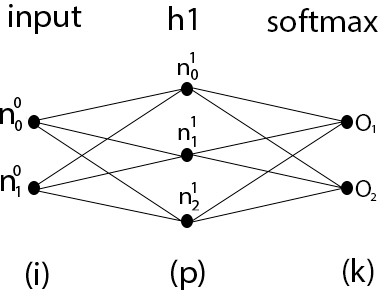
\includegraphics[scale=0.35]{imagenes/nn_1_capa.jpg}  
	\caption{Red Neuronal totalmente conectada con 1 capa oculta}
	\label{fig:nn_1_capa}
\end{figure}

La Figura \ref{fig:nn_1_capa} se compone de 'puntos' interconectados mediante líneas, representando neuronas y pesos que las conectan respectivamente. Cada punto corresponde a una neurona, y cada línea a un peso. \\
La Figura \ref{fig:nn_1_capa} presenta 3 capas (input, h1, softmax) que corresponden a capa de entrada, capa oculta $h_1$, y capa de salida respectivamente. El superíndice indica la capa a la que pertenece una neurona o peso, mientras que el subíndice indica el número del mismo en su respectiva capa. En el caso de los pesos, se requieren 2 subíndices para identificar a cada uno (pues un peso une 2 neuronas). \\
Así, la capa de entrada se compone de 2 neuronas ($n^{0}_0$ y $n^{0}_1$), la capa oculta $h_1$ tiene 3 neuronas ($n^1_{0}$, $n^1_{1}$, y $n^1_{2}$), y el peso $W^{i}_{jk}$ referencia al peso que une las neuronas $n^{i}_j$ y $n^{i+1}_k$.\\
De forma adicional, se recuerda que $Z_i$ representa la entrada $i$ de la capa SoftMax, y $O_i$ su salida.  

\subsubsection{Capa SoftMax}

\begin{figure}[H]
	\centering
	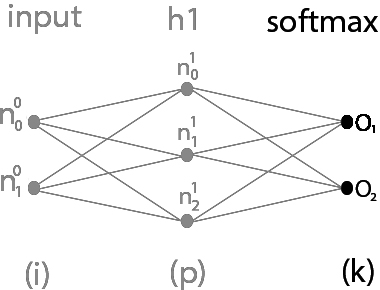
\includegraphics[scale=0.35]{imagenes/nn_1_capa_output.jpg}  
	\caption{Retropropagación en la capa softmax}
	\label{fig:nn_1_capa_output}
\end{figure}

Sea la neurona $n^i_j$, se define como $a^i_j$ el valor de dicha neurona antes de aplicar sobre ella su función de activación asociada, y $z^i_j$ el obtenido tras aplicarla. 

Tal y como se calculó previamente, el gradiente de la función de pérdida respecto a cada $Z_i$ viene dado por la fórmula \ref{gradiente_softmax}.


\subsubsection{Pesos capas h1-SoftMax}

\begin{figure}[H]
	\centering
	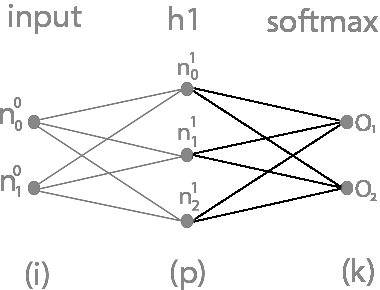
\includegraphics[scale=0.35]{imagenes/nn_1_capa_pesos_h1_output.jpg}  
	\caption{Retropropagación respecto a pesos entre la capa oculta y la capa SoftMax}
	\label{fig:nn_1_pesos_h1_output}
\end{figure}

Una vez calculado el gradiente hasta la entrada de la capa softmax, se puede calcular el gradiente respecto a cada peso $W^1_{pk}$ que se encuentra conectado a esta desde la capa anterior. Es decir, para cada $h^1_p\in h_1$, se calcula $\frac{dE(x)}{dW^1_{pk}}$. Usando la regla de la cadena, equivale a realizar lo ilustrado en las fórmulas \ref{grad_w1pk_1} y \ref{grad_w1pk_2}.

\begin{gather}
	\frac{\partial Z_k}{\partial W^1_{pk}} = \frac{\partial (z^1_p * W^1 _{pk}+ b^2_k)}{\partial W^1_{pk }} = z^1_p
	\label{grad_w1pk_1}
\end{gather}

\begin{gather}
	\frac{\partial E(x)}{\partial W^1_{pk }} =  gradiente\_Z_k * \frac{\partial Z_k}{\partial W^1_{pk }} = gradiente\_Z_k * z^1_p
	\label{grad_w1pk_2}
\end{gather}

\subsubsection{Sesgos capa softmax}

De la misma forma, se calcula el gradiente de la pérdida respecto a cada sesgo de las neuronas de la capa softmax tal y como se muestra en las fórmulas \ref{grad_b_h1_1}, \ref{grad_b_h1_2} y \ref{grad_b_h1_3}.

\begin{gather}
	\frac{\partial E}{\partial b^2_k} = \frac{\partial E}{\partial Z_k} * \frac{\partial Z_k}{b^2_k} \label{grad_b_h1_1} \\
	\frac{\partial Z_k }{\partial b^2_k } = \frac{\partial ([\sum_{c=1}^{P} z^1_c * W^1_{pk}] + b^2_k) }{\partial b^2_k } = 1 \label{grad_b_h1_2} \\
	\frac{\partial E}{\partial b^2_k} = gradiente\_Z_k \label{grad_b_h1_3}
\end{gather}

\subsubsection{Capa oculta h1}

\begin{figure}[H]
	\centering
	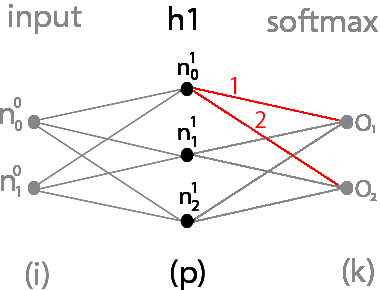
\includegraphics[scale=0.35]{imagenes/nn_caminos_posibles.jpg}  
	\caption{Imagen de los 'caminos' desde la capa softmax hasta la neurona $n^1_0$}
	\label{nn_caminos_posibles}
\end{figure}

En la figura \ref{nn_caminos_posibles} se muestra como hay más de un 'camino' desde la capa softmax hasta $n^1_p$. Por tanto, para obtener el gradiente de la pérdida respecto a $n^1_p$, habría que calcular la suma de todos los 'caminos' hacia este, tal y como se muestra en las fórmulas \ref{E_total_a1p} y \ref{deriv_Zk_z1p}. \\

\begin{gather}
	\frac{\partial E_{total}}{\partial a^1_p} = \sum_{k=1}^K \frac{\partial E_k}{\partial a^1_p} = \sum_{k=1}^K  gradiente\_Z_k * \frac{\partial Z_k}{\partial z^1_p} * \frac{\partial z^1_p}{\partial a^1_p}
	\label{E_total_a1p}
\end{gather}

\begin{gather}
	\frac{\partial Z_k}{\partial z^1_p} = \frac{\partial( [\sum_{c=1}^{P} z^1_c * W^1_{ck}] + b^2_k)}{\partial z^1_p} = W^1_{pk}
	\label{deriv_Zk_z1p}
\end{gather}

Para calcular dichos gradientes, se requiere calcular $\frac{\partial z^1_p}{\partial a^1_p}$. Como se mencionó anteriormente, ``a'' se refiere al valor de una neurona antes de aplicar la función de activación asociada, y ``z'' consiste en dicho valor tras aplicar la función de activación. Por tanto, para calcular $\frac{\partial z^1_p}{\partial a^1_p}$ se requiere saber dicha función de activación.

\begin{figure}[H]
	\centering
	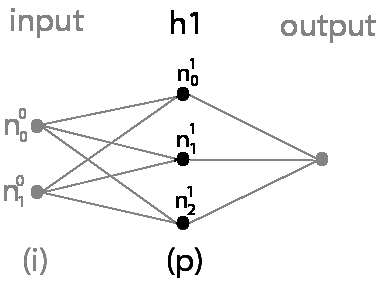
\includegraphics[scale=0.35]{imagenes/nn_1_capa_h1.jpg}  
	\caption{Retropropagación respecto a neuronas de la capa oculta h1}
	\label{fig:nn_1_capa_h1}
\end{figure}

En este ejemplo, en la capa oculta h1 se emplea la función de activación sigmoide, y su derivada viene dada por las fórmulas \ref{grad_sig_1} y \ref{grad_sig_2}. 

\begin{gather}
	sigmoide(x) = \frac{1}{1+e^{-x}} \label{grad_sig_1} \\
	sigmoide'(x) = \frac{sigmoide(x)}{1-sigmoide(x)} \label{grad_sig_2}
\end{gather}

De esta forma, ahora sí se puede calcular $\frac{\partial z^1_p}{\partial a^1_p}$, y se muestra en la fórmula \ref{deriv_z1p_a1p}.

\begin{gather}
	\frac{\partial z^1_ p}{\partial a^1_p} = \frac{\partial sigmoide(a^1_p)}{\partial a^1_p} = sigmoide(a^1_p)*(1-sigmoide(a^1_p))
	\label{deriv_z1p_a1p}
\end{gather}

Así, se retoma la fórmula \ref{E_total_a1p} mediante la aplicación de \ref{deriv_Zk_z1p} y \ref{deriv_z1p_a1p}, y se obtiene \ref{grad_E_a1p}.

\begin{gather}
	\frac{\partial E_{total}}{\partial a^1_p} = \sum_{k=1}^K  gradiente\_Z_k * W^1_{pk} * sigmoide(a^1_p)*(1-sigmoide(a^1_p)) \label{grad_E_a1p} \\
	\frac{\partial E_{total}}{\partial a^1_p} = gradiente\_h1_p
\end{gather}

\subsubsection{Pesos capas entrada-h1}

Una vez realizada la retropropagación hasta las neuronas de entrada de la capa oculta h1, se puede seguir con el proceso hacia la capa anterior (capa de entrada).

\begin{figure}[H]
	\centering
	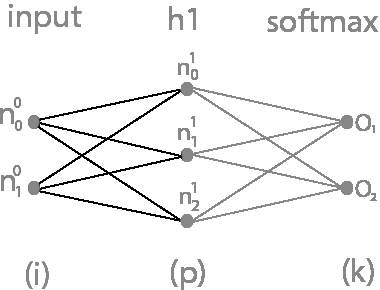
\includegraphics[scale=0.35]{imagenes/nn_1_capa_pesos_input_h1.jpg}  
	\caption{Retropropagación respecto a los pesos entre la capa de entrada y la capa oculta h1}
	\label{fig:nn_1_pesos_input_h1}
\end{figure}


\begin{gather}
	\frac{\partial a^1_p }{\partial W^0_{ip} } = \frac{\partial [\sum_{c=1}^{I} z^0_c * W^0_{cp}] + b^1_p)}{\partial W^0_{ip} } = z^0_i \label{grad_w0ip_1} \\
	\frac{\partial E}{\partial W^0_{ip}} = \frac{\partial E_{total} }{\partial a^1_p } * \frac{\partial a^1_p}{W^0_{ip}} \label{grad_w0ip_2} \\
	\frac{\partial E(x) }{\partial W^0_{ip} } = gradiente\_h1_p * \frac{\partial a^1_p }{\partial W^0_{ip} } = gradiente\_h1_p * z^0_i 
	\label{grad_w0ip_3}
\end{gather}

De forma similar a los pesos entre la capa oculta h1 y la capa softmax, se calcula el gradiente de la pérdida respecto a los pesos entre la capa de entrada y la capa oculta h1. El proceso se muestra mediante las fórmulas \ref{grad_w0ip_1}, \ref{grad_w0ip_2}, y \ref{grad_w0ip_3}.

\subsubsection{Sesgos capa h1}

\begin{gather}
	\frac{\partial E}{\partial b^1_p} = \frac{\partial E_{total} }{\partial a^1_p } * \frac{\partial a^1_p}{b^1_p} \label{grad_b1p_1} \\
	\frac{\partial a^1_p }{\partial b^1_p } = \frac{\partial ([\sum_{c=1}^{I} z^0_c * W^0_{ip}] + b^1_p) }{\partial b^1_p } = 1 \label{grad_b1p_2} \\
	\frac{\partial E}{\partial b^1_p} = gradiente\_h1_p
	\label{grad_b1p_3}
\end{gather}

Del mismo modo, las figuras \ref{grad_b1p_1}, \ref{grad_b1p_2}, y \ref{grad_b1p_3} muestran el cálculo del gradiente respecto a los sesgos de la capa oculta h1.

\subsubsection{Capa de entrada}

\begin{figure}[H]
	\centering
	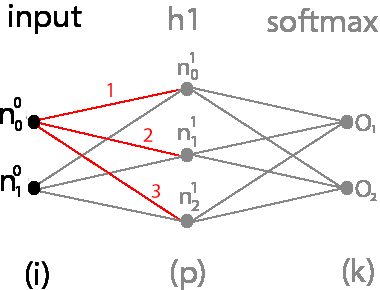
\includegraphics[scale=0.35]{imagenes/nn_caminos_posibles_input.jpg}  
	\caption{Imagen de los 'caminos' desde la capa oculta h1 hasta $n^0_0$}
	\label{nn_caminos_posibles_input}
\end{figure}

Por último, en esta sección se calcula el gradiente respecto a las neuronas de entrada de la capa de entrada. Normalmente no sería necesario calcular estos gradientes, pero como el objetivo es crear una CNN, esta red totalmente conectada estará enlazada a capas convolucionales y de agrupación máxima, por lo que es necesario calcular dichos gradientes para poder seguir calculando la retropropagación en dichas capas anteriores a esta.

\begin{gather}
	\frac{\partial E_{total}}{\partial a^0_i} = \sum_{p=1}^P \frac{\partial E_{total}}{\partial a^1_p} * \frac{\partial a^1_p}{\partial z^0_i} * \frac{\partial z^0_i}{\partial a^0_i} \label{grad_a_1} \\
	\frac{\partial a^1_p }{\partial z^0_i } = \frac{\partial ([\sum_{c=1}^{I} z^0_c * W^0_{ip}] + b^1_p) }{\partial z^0_i } = W^0_{ip} \label{grad_a_2}
\end{gather}

\begin{figure}[H]
	\centering
	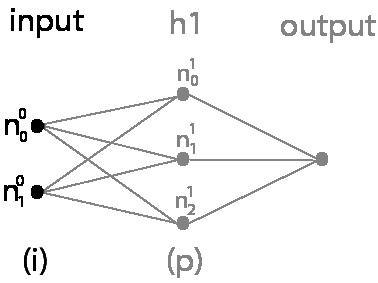
\includegraphics[scale=0.35]{imagenes/nn_1_capa_input.jpg}  
	\caption{Retropropagación en la capa input}
	\label{fig:nn_1_capa_input}
\end{figure}

Como la capa input no presenta ninguna función de activación asociada, $z^0_i$ es igual $a^0_i$. \\

\begin{gather}
	\frac{\partial z^0_i }{\partial a^0_i } = 1 \\
	\frac{\partial E_{total}}{\partial a^0_i} = \sum_{p=1}^{P} gradiente\_h1_p
\end{gather}

\subsection{Retropropagación con 2 capas ocultas}

\begin{figure}[H]
	\centering
	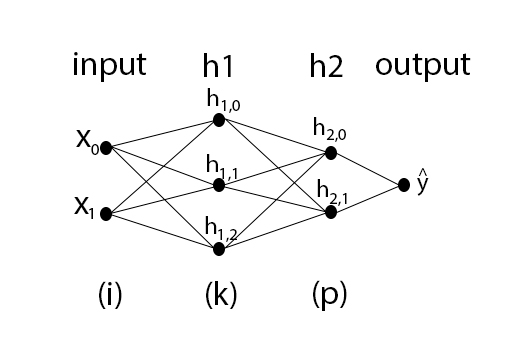
\includegraphics[scale=0.35]{imagenes/nn_2_capas.jpg}  
	\caption{Red Neuronal totalmente conectada con 2 capas ocultas}
	\label{fig:nn_2_capas}
\end{figure}

A diferencia del apartado anterior, en este caso se emplea una red totalmente conectada con 2 capas ocultas (h1 y h2), tal y como se muestra en la Figura \ref{fig:nn_2_capas}. \\

\subsubsection{Capa SoftMax}

\begin{figure}[H]
	\centering
	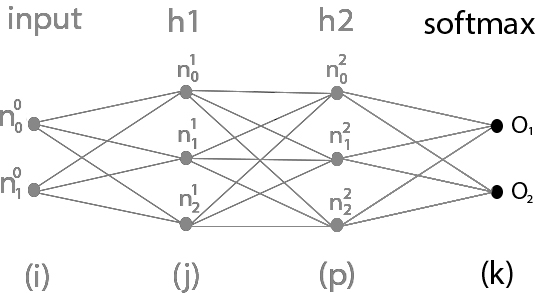
\includegraphics[scale=0.35]{imagenes/nn_2_capa_output.jpg}  
	\caption{Retropropagación en la capa softmax}
\end{figure}

De igual forma que en los casos anteriores, el gradiente de la función de pérdida respecto a cada $Z_i$ viene dado por la fórmula \ref{gradiente_softmax}. Por tanto, no se repetirán los cálculos. \\

\subsubsection{Pesos capas h2-SoftMax}

\begin{figure}[H]
	\centering
	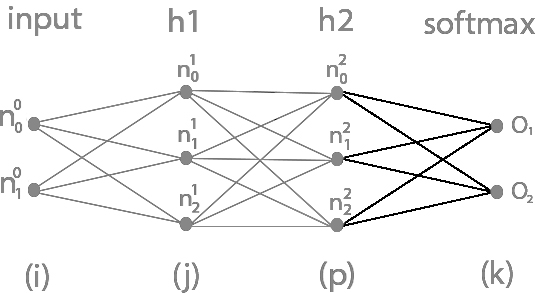
\includegraphics[scale=0.35]{imagenes/nn_2_capa_pesos_h2_output.jpg}  
	\caption{Retropropagación respecto a los pesos entre la capa oculta h2 y la capa SoftMax}
\end{figure}

Se realiza el cálculo del gradiente de la función de pérdida respecto a cada peso $W^2_{pk}$ que une las neuronas de la capa oculta h2 con las de la capa softmax. \\

\begin{gather}
	\frac{\partial Z_k}{\partial W^2_{pk}} = \frac{\partial (z^2_p * W^2 _{pk} + b^3_k)}{\partial W^2_{pk }} = z^2_p 
	\label{grad_w2pk_1}
\end{gather}

\begin{gather}
	\frac{\partial E(x)}{\partial W^2_{pk }} =  gradiente\_Z_k * \frac{\partial Z_k}{\partial W^2_{pk }} = gradiente\_Z_k * z^2_p
	\label{grad_w2pk_2}
\end{gather}

Como es de esperar, las fórmulas \ref{grad_w2pk_1} y \ref{grad_w2pk_2} son casi idénticas a \ref{grad_w1pk_1} y \ref{grad_w1pk_2} respectivamente, salvo por el superíndice empleado (1 $\neq$ 2). Esto tiene sentido pues esta parte también es común al apartado anterior.

\subsubsection{Sesgos capa softmax}

\begin{gather}
	\frac{\partial E}{\partial b^3_k} = \frac{\partial E}{\partial Z_k} * \frac{\partial Z_k}{b^3_k} \label{grad_b_h2_1} \\
	\frac{\partial Z_k }{\partial b^3_k } = \frac{\partial ([\sum_{c=1}^{P} z^2_c * W^2_{pk}] + b^3_k) }{\partial b^3_k } = 1 \label{grad_b_h2_2} \\
	\frac{\partial E}{\partial b^3_k} = gradiente\_Z_k \label{grad_b_h2_3}
\end{gather}

De igual forma, el cálculo del gradiente de la pérdida respecto a los sesgos de la capa softmax también permanece inalterado, por lo que la única diferencia entre las fórmulas $\{$\ref{grad_b_h2_1}, \ref{grad_b_h2_2}, \ref{grad_b_h2_3}$\}$ y $\{$\ref{grad_b_h1_1}, \ref{grad_b_h1_2}, \ref{grad_b_h1_3}$\}$ son los superíndices empleados.

\subsubsection{Capa oculta h2}

\begin{figure}[H]
	\centering
	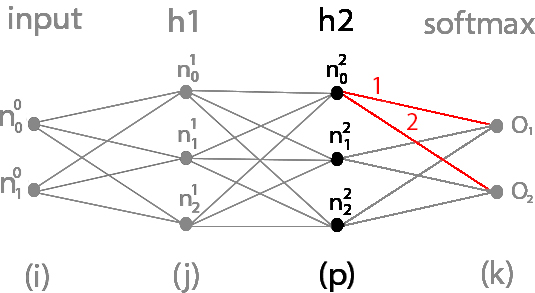
\includegraphics[scale=0.35]{imagenes/nn_h2_caminos_posibles.jpg}  
	\caption{Imagen de los 'caminos' desde la capa softmax hasta $n^2_0$}
	\label{nn_h2_caminos_posibles}
\end{figure}

Tal y como se comentó anteriormente, hay más de un 'camino' desde la capa softmax hasta $n^2_p$. Por tanto, para obtener el gradiente de la pérdida respecto a cada $n^2_p$, habría que calcular la suma de todos los ellos, tal y como se muestra en las fórmulas \ref{E_total_a2p} y \ref{deriv_Zk_z2p}. \\

\begin{gather}
	\frac{\partial E_{total}}{\partial a^2_p} = \sum_{k=1}^K \frac{\partial E_k}{\partial a^2_p} = \sum_{k=1}^K  gradiente\_Z_k * \frac{\partial Z_k}{\partial z^2_p} * \frac{\partial z^2_p}{\partial a^2_p}
	\label{E_total_a2p}
\end{gather}

\begin{gather}
	\frac{\partial Z_k}{\partial z^2_p} = \frac{\partial( [\sum_{c=1}^{P} z^2_c * W^2_{ck}] + b^3_k)}{\partial z^2_p} = W^2_{pk}
	\label{deriv_Zk_z2p}
\end{gather}

\begin{figure}[H]
	\centering
	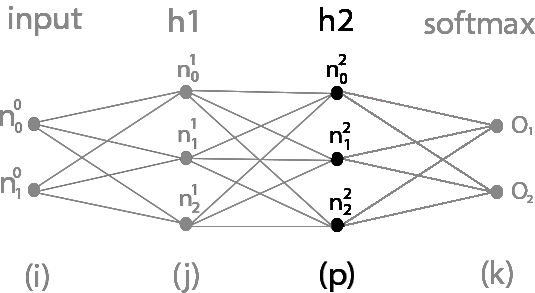
\includegraphics[scale=0.35]{imagenes/nn_2_capa_h2.jpg}  
	\caption{Retropropagación en la capa oculta h2}
	\label{fig:nn_2_capa_h2}
\end{figure}

Por coincidir con el ejemplo anterior, en la última capa oculta (h2 en este caso) se vuelve a emplear sigmoide como función de activación. Así, se vuelve a mostrar la derivada de dicha función en las fórmulas \ref{grad_sig_h2_1} y \ref{grad_sig_h2_2} por facilitar la comprensión del lector.

\begin{gather}
	sigmoide(x) = \frac{1}{1+e^{-x}} \label{grad_sig_h2_1} \\
	sigmoide'(x) = \frac{sigmoide(x)}{1-sigmoide(x)} \label{grad_sig_h2_2}
\end{gather}


Empleando la derivada de sigmoide se consigue la fórmula \ref{deriv_z2p_a2p}.

\begin{gather}
	\frac{\partial z^2_ p}{\partial a^2_p} = \frac{\partial sigmoide(a^2_p)}{\partial a^2_p} = sigmoide(a^2_p)*(1-sigmoide(a^2_p))
	\label{deriv_z2p_a2p}
\end{gather}

Tras ello, se retoma la fórmula \ref{E_total_a2p} mediante la aplicación de \ref{deriv_Zk_z2p} y \ref{deriv_z2p_a2p} para obtener \ref{grad_E_a2p}.

\begin{gather}
	\frac{\partial E_{total}}{\partial a^2_p} = \sum_{k=1}^K  gradiente\_Z_k * W^2_{pk} * sigmoide(a^2_p)*(1-sigmoide(a^2_p)) \label{grad_E_a2p} \\
	\frac{\partial E_{total}}{\partial a^2_p} = gradiente\_h2_p
\end{gather}

Una vez más, la fórmula obtenida (\ref{grad_E_a2p}) coindice con la calculada previamente (\ref{grad_E_a1p}) a excepción de los superíndices empleados. \\

\subsubsection{Pesos capas h1-h2}

\begin{figure}[H]
	\centering
	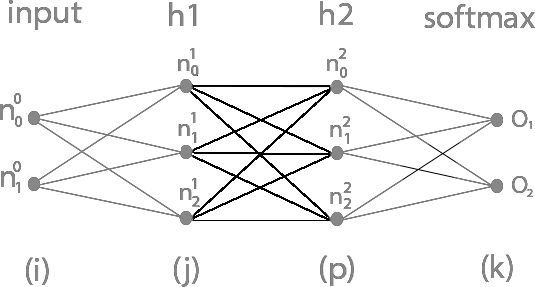
\includegraphics[scale=0.35]{imagenes/nn_2_capa_pesos_h1_h2.jpg}  
	\caption{Retropropagación respecto a los pesos entre las capas ocultas h1 y h2}
	\label{fig:nn_2_pesos_h1_h2}
\end{figure}


\begin{gather}
	\frac{\partial a^2_p }{\partial W^1_{jp} } = \frac{\partial [\sum_{c=1}^{J} z^1_c * W^1_{cp}] + b^2_p)}{\partial W^1_{jp} } = z^1_j \\
	\frac{\partial E}{\partial W^1_{jp}} = \frac{\partial E_{total} }{\partial a^2_p } * \frac{\partial a^2_p}{W^1_{jp}} \\
	\frac{\partial E(x) }{\partial W^1_{jp} } = gradiente\_h2_p * \frac{\partial a^2_p }{\partial W^1_{jp} } = gradiente\_h2_p * z^1_j 
	\label{grad_w1jp}
\end{gather}

Como esta parte también es común al caso anterior, la fórmula \ref{grad_w1jp} vuelve a coincidir con \ref{grad_w0ip_3}


\subsubsection{Sesgos capa h2}

\begin{gather}
	\frac{\partial E}{\partial b^2_p} = \frac{\partial E_{total} }{\partial a^2_p } * \frac{\partial a^2_p}{b^2_p} \\
	\frac{\partial a^2_p }{\partial b^2_p } = \frac{\partial ([\sum_{c=1}^{J} z^1_c * W^1_{jp}] + b^2_p) }{\partial b^2_p } = 1 \\
	\frac{\partial E}{\partial b^2_p} = gradiente\_h2_p
	\label{grad_b2p}
\end{gather}

Una vez más, la fórmula \ref{grad_b2p} coincide con \ref{grad_b1p_3}. Es importante notar aquellas partes comunes que comparten ambos casos de cara a una posterior generalización del modelo y poder automatizar dichos cálculos.

\subsubsection{Capa oculta h1}

\begin{figure}[H]
	\centering
	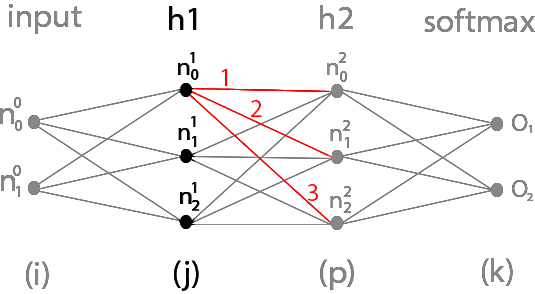
\includegraphics[scale=0.35]{imagenes/nn_h1_caminos_posibles.jpg}  
	\caption{'Caminos' desde la capa softmax hasta $n^1_0$}
	\label{nn_h1_caminos_posibles}
\end{figure}

De igual forma que se realizó en la capa h2, se calcula la suma de todos los 'caminos' hacia cada neurona $n^1_j$. \\

\begin{gather}
	\frac{\partial E_{total}}{\partial a^1_j} = \sum_{k=1}^K \frac{\partial E_k}{\partial a^1_j} = \sum_{p=1}^P  gradiente\_h2_p * \frac{\partial a^2_p}{\partial z^1_j} * \frac{\partial z^1_j}{\partial a^1_j} \\
	\frac{\partial a^2_p}{\partial z^1_j} = \frac{\partial( [\sum_{c=1}^{J} z^1_c * W^1_{cp}] + b^2_p)}{\partial z^1_j} = W^1_{jp}
\end{gather}

Como es de esperar, se calcula el gradiente respecto a cada neurona de la capa h1 teniendo en cuenta cada `camino' del gradiente desde la capa siguiente (h2).

\begin{figure}[H]
	\centering
	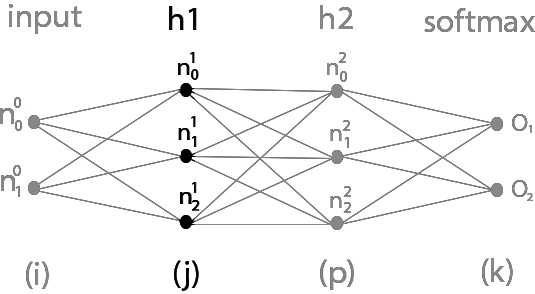
\includegraphics[scale=0.35]{imagenes/nn_2_capa_h1.jpg}  
	\caption{Retropropagación en la capa oculta h1}
\end{figure}

En este caso, en la capa oculta h1 se emplea la función de activación ReLU, y su derivada viene dada por la fórmula \ref{deriv_relu}. 

\begin{gather}
	ReLU(x) = max(0, x) \\
	ReLU'(x) = 1\ si\ x>0,\ 0\ en\ caso\ contrario
	\label{deriv_relu}
\end{gather}

Esta se emplea para obtener el gradiente $\frac{\partial z^1_ j}{\partial a^1_j}$, así como seguir la retropropagación por la capa, tal y como se muestra en las siguientes fórmulas (\ref{grad_E_a1j_1}, \ref{grad_E_a1j_2}, y \ref{grad_E_a1j_3}).


\begin{gather}
	\frac{\partial z^1_ j}{\partial a^1_j} = 1\ si\ x>0,\ 0\ en\ caso\ contrario \label{grad_E_a1j_1} \\
	\frac{\partial E_{total}}{\partial a^1_j} = \sum_{p=1}^P  gradiente\_h2_p * W^1_{jp} * ReLU'(a^1_j) \label{grad_E_a1j_2} \\
	\frac{\partial E_{total}}{\partial a^1_j} = gradiente\_h1_j
	\label{grad_E_a1j_3}
\end{gather}

Una vez más, el proceso de obtención de la fórmula \ref{grad_E_a1j_2} es muy parecido al realizado para casos anteriores aunque esta capa sea algo ``nuevo'' respecto a la sección anterior. \\


\subsubsection{Pesos capa input-h1}

\begin{figure}[H]
	\centering
	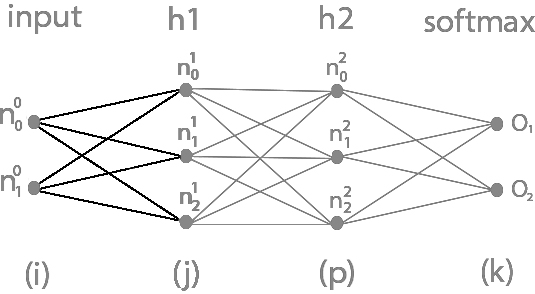
\includegraphics[scale=0.35]{imagenes/nn_2_capa_pesos_input_h1.jpg}  
	\caption{Retropropagación respecto a los pesos entre la capa de entrada (input) y la capa oculta h1}
	\label{fig:nn_2_pesos_input_h1}
\end{figure}


\begin{gather}
	\frac{\partial a^1_j }{\partial W^0_{ij} } = \frac{\partial ([\sum_{c=1}^{I} z^0_c * W^0_{cj}] + b^1_j)}{\partial W^0_{ij} } = z^0_i \label{grad_w0ip_h2_1} \\
	\frac{\partial E}{\partial W^0_{ij}} = \frac{\partial E_{total} }{\partial a^1_j } * \frac{\partial a^1_j}{W^0_{ij}} \label{grad_w0ip_h2_2} \\
	\frac{\partial E(x) }{\partial W^0_{ij} } = gradiente\_h1_j * \frac{\partial a^1_j }{\partial W^0_{ij} } = gradiente\_h1_j * z^0_i \label{grad_w0ip_h2_3}
\end{gather}

Aquí se aprecia como las fórmulas $\{$\ref{grad_w0ip_h2_1}, \ref{grad_w0ip_h2_2}, \ref{grad_w0ip_h2_3} $\}$ son iguales a $\{$\ref{grad_w0ip_1}, \ref{grad_w0ip_2}, \ref{grad_w0ip_3} $\}$ excepto por el subíndice empleado (j $\neq$ p). Aunque los valores analíticos no sean los mismos pues las arquitecturas son diferentes, la notación empleada se ha creado con el objetivo de facilitar la visualización y comprensión de la gran capacidad de automatización en capas totalmente conectadas.

\subsubsection{Sesgos capa h1}

\begin{gather}
	\frac{\partial E}{\partial b^1_j} = \frac{\partial E_{total} }{\partial a^1_j } * \frac{\partial a^1_j}{b^1_j} \label{grad_b1j_h2_1} \\
	\frac{\partial a^1_j }{\partial b^1_j } = \frac{\partial ([\sum_{c=1}^{I} z^0_c * W^0_{ij}] + b^1_j) }{\partial b^1_j } = 1 \label{grad_b1j_h2_2} \\
	\frac{\partial E}{\partial b^1_j} = gradiente\_h1_j
	\label{grad_b1j_h2_3}
\end{gather}

De esta forma, las fórmulas $\{$\ref{grad_b1j_h2_1}, \ref{grad_b1j_h2_2}, \ref{grad_b1j_h2_3} $\}$ y $\{$\ref{grad_b1p_1}, \ref{grad_b1p_2}, \ref{grad_b1p_3} $\}$ también coincide en todo menos en el subíndice (j $\neq$ p).

\subsubsection{Capa input}

\begin{figure}[H]
	\centering
	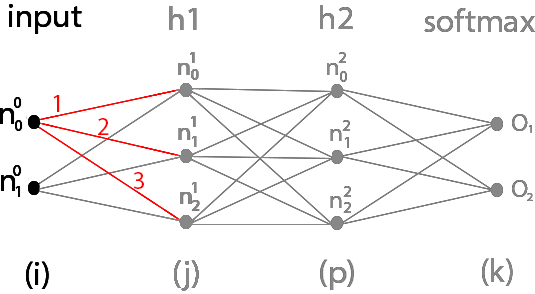
\includegraphics[scale=0.35]{imagenes/nn_2_capas_caminos_posibles_input.jpg}  
	\caption{'Caminos' desde la capa oculta h1 hasta $n^0_0$}
	\label{nn_2_capas_caminos_posibles_input}
\end{figure}

\begin{gather}
	\frac{\partial E_{total}}{\partial a^0_i} = \sum_{j=1}^J \frac{\partial E_{total}}{\partial a^1_j} * \frac{\partial a^1_j}{\partial z^0_i} * \frac{\partial z^0_i}{\partial a^0_i} \label{grad_a_h2_1} \\
	\frac{\partial a^1_j }{\partial z^0_i } = \frac{\partial ([\sum_{c=1}^{I} z^0_c * W^0_{ij}] + b^1_j) }{\partial z^0_i } = W^0_{ij} \label{grad_a_h2_2}
\end{gather}

Aquí también se aprecia como a diferencia de los subíndices empleados, las fórmulas $\{$\ref{grad_a_h2_1}, \ref{grad_a_h2_2} $\}$    y    $\{$\ref{grad_a_1}, \ref{grad_a_2}$\}$ son exactamente iguales.

\begin{figure}[H]
	\centering
	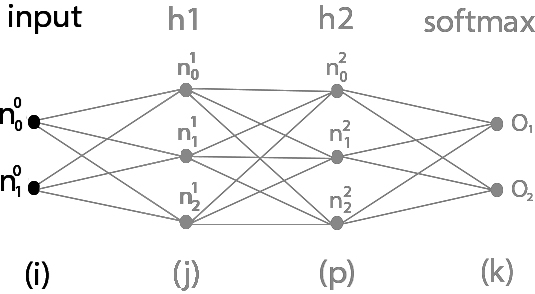
\includegraphics[scale=0.35]{imagenes/nn_2_capa_input.jpg}  
	\caption{Retropropagación en la capa input}
	\label{fig:nn_2_capa_input}
\end{figure}

Como la capa input no presenta ninguna función de activación asociada, $z^0_i$ es igual $a^0_i$, (igual que en el caso anterior). \\

\begin{gather}
	\frac{\partial z^0_i }{\partial a^0_i } = 1 \\
	\frac{\partial E_{total}}{\partial a^0_i} = \sum_{p=1}^{P} gradiente\_h1_p
\end{gather}

\subsection{Conclusiones}
Se definen como capas ocultas ``intermedias'' todas menos la última de ellas. Tal y como se ha mostrado anteriormente, comparten la mayoría del cálculo en cuanto a retropopagación. De esta forma, se puede dividir una red neuronal totalmente conectada en 4 grupos $\{$capa input, capas ocultas intermedias, última capa oculta, capa de salida o capa softmax$\}$. \\
A continuación se realiza el cálculo necesario para la retropropagación de una capa de neuronas `l' determinada. Suponemos que la capa l+1 tiene Q neuronas, la capa l-1 tiene K neuronas, y todas las capas ocultas intermedias usan ReLU como función de activación. \\

\subsubsection{Gradiente respecto a la entrada de la capa}

\begin{figure}[H]
	\centering
	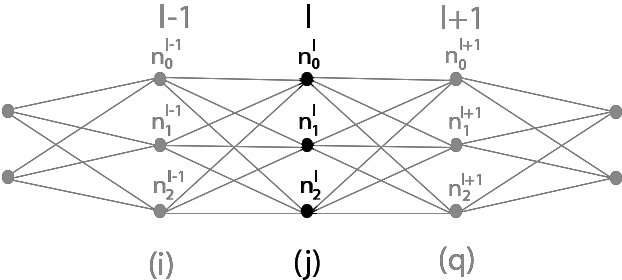
\includegraphics[scale=0.35]{imagenes/conclusion_capa_l.jpg}  
	\caption{Retropropagación en la capa l}
	\label{fig:conclusion_capa_l}
\end{figure}

\begin{gather}
	\frac{\partial E_{total}}{\partial a^l_j} = \sum_{q=1}^Q \frac{\partial E_{total}}{\partial a^{l+1}_q} * \frac{\partial a^{l+1}_q}{\partial z^l_j} * \frac{\partial z^l_j}{\partial a^l_j} \label{grad_input_l_1} \\
	\frac{\partial a^{l+1}_j }{\partial z^l_j } = \frac{\partial ([\sum_{c=1}^{K} z^l_c * W^l_{ij}] + b^{l+1}_j) }{\partial z^l_j } = W^l_{ij} \label{grad_input_l_2} \\
	\frac{\partial z^l_j}{\partial a^l_j} = ReLU'(a^l_j) \label{grad_input_l_3} \\
	\frac{\partial E_{total}}{\partial a^l_j} = \sum_{q=1}^Q  gradiente\_h_{{l+1}_q} * W^l_{ij} * ReLU'(a^l_j) \label{grad_input_l_4} \\
	\frac{\partial E_{total}}{\partial a^l_j} = gradiente\_h_{l_j} \label{grad_input_l_5}
\end{gather}

Las fórmulas \ref{grad_input_l_1}, \ref{grad_input_l_2}, \ref{grad_input_l_3},  \ref{grad_input_l_4}, y \ref{grad_input_l_5} muestran el cálculo genérico requerido para obtener el gradiente de la pérdida respecto a la entrada de una capa oculta intermedia `l'.

\subsubsection{Gradiente respecto a los pesos}

\begin{figure}[H]
	\centering
	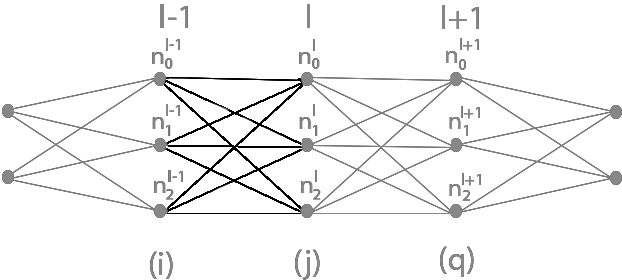
\includegraphics[scale=0.35]{imagenes/conclusion_pesos.jpg}  
	\caption{Retropropagación respecto a los pesos entre la capa l-1 y l}
	\label{fig:conclusion_pesos}
\end{figure}

\begin{gather}
	\frac{\partial E}{\partial W^{l-1}_{ij}} = \frac{\partial E_{total} }{\partial a^l_j } * \frac{\partial a^l_j}{W^{l-1}_{ij}} \label{grad_w_l_1} \\
	\frac{\partial a^l_j }{\partial W^{l-1}_{ij} } = \frac{\partial ([\sum_{c=1}^{K} z^{l-1}_c * W^{l-1}_{cj}] + b^l_j)}{\partial W^{l-1}_{ij} } = z^{l-1}_i \label{grad_w_l_2} \\
	\frac{\partial E(x) }{\partial W^{l-1}_{ij} } = gradiente\_h_{l_j} * \frac{\partial a^l_j }{\partial W^{l-1}_{ij} } = gradiente\_h_{l_j} * z^{l-1}_i \label{grad_w_l_3}
\end{gather}

Las fórmulas \ref{grad_w_l_1}, \ref{grad_w_l_2}, y \ref{grad_w_l_3} muestran el cálculo requerido para obtener el gradiente de la pérdida respecto a los pesos entre las capas ocultas genéricas l y l-1.

\subsubsection{Gradiente respecto a sesgos}

\begin{gather}
	\frac{\partial E}{\partial b^l_j} = \frac{\partial E_{total} }{\partial a^l_j } * \frac{\partial a^l_j}{b^l_j} \label{grad_b_l_1} \\
	\frac{\partial a^l_j }{\partial b^l_j } = \frac{\partial ([\sum_{c=1}^{K} z^{l-1}_c * W^{l-1}_{ij}] + b^l_j) }{\partial b^l_j } = 1 \label{grad_b_l_2} \\
	\frac{\partial E}{\partial b^l_j} = gradiente\_h_{l_j} \label{grad_b_l_3}
\end{gather}

Las fórmulas \ref{grad_b_l_1}, \ref{grad_b_l_2}, y \ref{grad_b_l_3} muestran el cálculo requerido para obtener el gradiente de la pérdida respecto a los sesgos de la capa oculta genérica l.

\section{Paralelización mediante OpenMP}

\subsubsection{Tipos de paralelismo}

El entrenamiento de una red neuronal convolucional (CNN) se puede paralelizar de distintas formas. Si el modelo se reparte entre varios ordenadores que son entrenados con los mismos datos, se denomina \textbf{paralelismo del modelo} (una capa por computador, por ejemplo). Sin embargo, si se distribuyen los datos entre múltiples nodos pero se emplea el mismo modelo para entrenar, se denomina \textbf{paralelismo de datos}. \\

\subsubsection{Paralelismo en SGD}
\begin{algorithm}[H]
	\caption{Descenso del gradiente estocástico} 
	\begin{algorithmic}
		\State Datos de entrenamiento $D=\{(x_1, y_1), (x_2, y_2), ..., (x_N, y_N)\}$.
		
		\For{cada trabajador $t =0, ..., T-1$ en paralelo}
		\For{época $p\in\{0, ..., P-1\}$}
			\State Desordenar vector de datos D.
				\For{cada mini batch $m =0, ..., M-1$}
					\State Inicializar $gradientes^t$ a 0.
					\State Reparto de datos del batch m al trabajador t
					\State Realizar propagación hacia delante
					\State Obtener error total con la función de pérdida
					\State Realizar propagación hacia detrás y obtener $gradientes^t$ 
					\State de cada parámetro del modelo.
					
					\State Acumular gradientes obtenidos por cada trabajador t.
					\State Actualizar parámetros.
					
				\EndFor
			\EndFor
		\EndFor
	\end{algorithmic}
\end{algorithm}

La naturaleza iterativa del algoritmo del descenso del gradiente estocástico puede parecer un obstáculo ante la paralelización del entrenamiento del modelo, pues la iteración i se basa en el resultado obtenido en la iteración i-1. Sin embargo, tal y como se indica en \cite{CNN_parallel_Stanford}, \cite{CNN_parallel_International_Conference}, y \cite{CNN_parallel_Ome_Weird_Trick}, existe una forma de aplicar paralelismo en cada iteración. \\
En cada época se entrena al modelo con M subconjuntos de $N_m$ datos disjuntos entre ellos de forma que, dados T ``trabajadores'' o procesos paralelos, se puede dividir cada mini-batch a su vez en T subconjuntos de $\frac{N_m}{T}$ datos y asignar cada uno a un trabajador distinto.\\
Siguiendo el mismo razonamiento, se reparten los datos de entrenamiento entre los distintos trabajadores T tanto para realizar la propagación hacia delante como para la posterior retropropagación. En el caso de la retropropagación, se deberá acumular el gradiente de la pérdida respecto a cada parámetro obtenido por cada trabajor, y una vez en posesión de dicho gradiente `total' se procederá a la actualización de los parámetros del modelo.

\section{Retropropagación en redes neuronales convolucionales}

\begin{figure}[H]
	\centering
	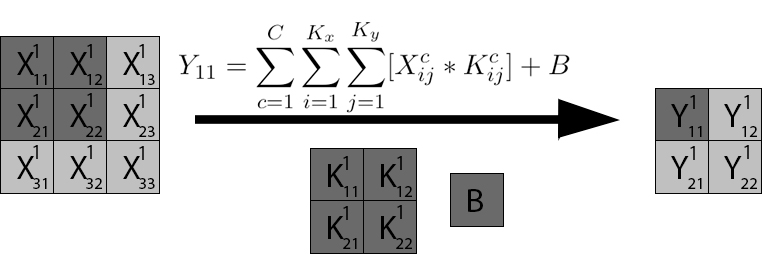
\includegraphics[width=0.8\linewidth]{imagenes/conv_ejemplo_backprop_1.jpg} 
	\caption{Ejemplo de propagación hacia delante en una capa convolucional}
	\label{fig:ejemplo_forward_prop_convolucional}
\end{figure}

La figura \ref{fig:ejemplo_forward_prop_convolucional} muestra el ejemplo de propagación hacia delante que se empleará en esta sección. En él, C indica el número de canales de profundidad del volumen de entrada X, mientras que $K_x$ y $K_y$ hacen referencia al número de filas y columnas del kernel K empleado, respectivamente. \\
Siguiendo la notación empleada en secciones anteriores, se denotará como $A^c_{ij}$ al valor $X^c_{ij}$ antes de aplicar sobre él su función de activación asociada, y $Z^c_{ij}$ una vez esta sea aplicada.

\subsubsection{Sumatoria de gradientes}

\begin{gather}
	\frac{\partial E}{\partial K^c_{11}} = \sum_{i=1}^{I}\sum_{j=1}^{J}  [\frac{\partial E}{\partial Y^c_{ij}} * \frac{\partial Y^c_{ij}}{\partial K^c_{11}}] \\
	\frac{\partial E}{\partial X^c_{11}} = \sum_{i=1}^{I}\sum_{j=1}^{J}  [\frac{\partial E}{\partial Y^c_{ij}} * \frac{\partial Y^c_{ij}}{\partial Z^c_{11}} * \frac{\partial Z^c_{ij}}{\partial A^c_{11}}] 
\end{gather}

Para calcular el gradiente de la función de error respecto a cada peso $K_{xy}$ o entrada $X_{xy}$, se deberá realizar una sumatoria del mismo respecto a cada valor de salida de dicha convolución. En el caso de los pesos de un canal de profundidad $c \in C$, cada uno se empleó en el cálculo de cada valor $Y^c_{ij}$. En el caso de la entrada, hay valores $x \in X $ que se emplearon en el cálculo de distintos $\{y_1, y_2\} \in Y$. Esto se vio anteriormente con detalle en la sección \ref{intro_CNN}.

\subsubsection{Gradiente de $Y^c_{11}$}

\begin{gather}
	Y^c_{11} = Z^c_{11} * K^c_{11} + Z^c_{12} * K^c_{12} + Z^c_{21} * K^c_{21} + Z^c_{22} * K^c_{22} \label{grad_y11_k_11} \\
	\frac{\partial Y^c_{11}}{\partial K^c_{xy}} = \frac{\partial (Z^c_{11} * K^c_{11} + Z^c_{12} * K^c_{12} + Z^c_{21} * K^c_{21} + Z^c_{22} * K^c_{22})}{\partial K^c_{xy}} \label{grad_y11_k_12} \\
	\frac{\partial Y^c_{11}}{\partial K^c_{11}} = Z^c_{11}, \hspace{10mm} \frac{\partial Y^c_{11}}{\partial K^c_{12}} = Z^c_{12} \label{grad_y11_k_21}\\
	\frac{\partial Y^c_{11}}{\partial K^c_{21}} = Z^c_{21}, \hspace{10mm} \frac{\partial Y^c_{11}}{\partial K^c_{22}} = Z^c_{22} \label{grad_y11_k_22}
\end{gather}

\begin{gather}
	\frac{\partial Y^c_{11}}{\partial Z^c_{11}} = K^c_{11}, \hspace{10mm} \frac{\partial Y^c_{11}}{\partial Z^c_{12}} = K^c_{12}, \hspace{10mm} \frac{\partial Y^c_{11}}{\partial Z^c_{13}} = 0 \label{grad_y11_z_1} \\
	\frac{\partial Y^c_{11}}{\partial Z^c_{21}} = K^c_{21}, \hspace{10mm} \frac{\partial Y^c_{11}}{\partial Z^c_{22}} = K^c_{22}, \hspace{10mm} \frac{\partial Y^c_{11}}{\partial Z^c_{23}} = 0 \label{grad_y11_z_2} \\
	\frac{\partial Y^c_{11}}{\partial Z^c_{31}} = 0, \hspace{15mm} \frac{\partial Y^c_{11}}{\partial Z^c_{32}} = 0, \hspace{15mm} \frac{\partial Y^c_{11}}{\partial Z^c_{33}} = 0 \label{grad_y11_z_3}
\end{gather}

La fórmula \ref{grad_y11_k_11} muestra una descomposición de $Y^c_{11}$ en términos de $Z$ y $K$. Esto resulta útil para calcular tanto el gradiente respecto a Z (fórmulas \ref{grad_y11_z_1}, \ref{grad_y11_z_2}, \ref{grad_y11_z_3}) como respecto a K (fórmulas \ref{grad_y11_k_12}, \ref{grad_y11_k_21}, \ref{grad_y11_k_22}). De esta forma, se calcula el gradiente de $Y^c_{11}$ respecto a cada parámetro de la capa convolucional. \\
Cabe destacar que para realmente calcular el gradiente respecto a cada valor del volumen de entrada (X), se debería calcular también la derivada de la función de activación asociada a dicha capa. Es decir, $\frac{\partial Z}{\partial A}$. Sin embargo, como este proceso ya se ha visto varias veces en secciones anteriores, se omitirá (por ahora) junto con el cálculo del gradiente respecto al sesgo de cada capa. El objetivo de ello reside en la eliminación de cálculos redundantes y centrar la atención en los aspectos importantes y novedosos. Aun así, todos los cálculos mostrados en esta documentación (y más) se encuentran en el código correspondiente, pues se recuerda que todo este conocimiento se ha llevado a la práctica y por ello comprobado su correcto funcionamiento. \\
Además, como todo se ha hecho a mano por la misma persona, la mayoría de las variables y/o índices coinciden a la perfección o son muy parecidas en la documentación y en el código, por lo que cualquier lector con conocimientos básicos de programación podría entender gran parte de las implementaciones desarrolladas en este proyecto.

\subsubsection{Gradiente de $Y^c_{12}$}

\begin{figure}[H]
	\centering
	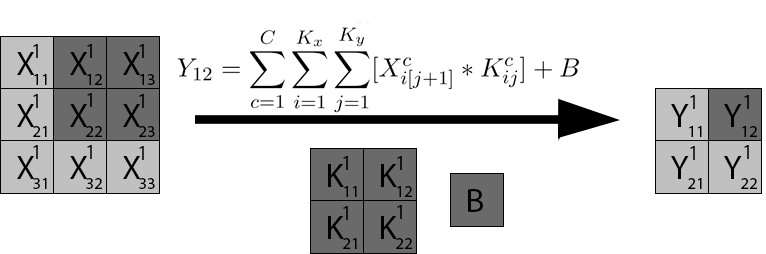
\includegraphics[width=1\linewidth]{imagenes/conv_ejemplo_backprop_2.jpg} 
	\caption{Cálculo de $Y^c_{12}$ mediante propagación hacia delante en una capa convolucional}
	\label{fig:ejemplo_2_forward_prop_convolucional}
\end{figure}

Del mismo modo, se calcula el gradiente de $Y^c_{12}$ respecto a cada peso (\ref{grad_y12_k_1} y \ref{grad_y12_k_2})

\begin{gather}
	Y^c_{12} = Z^c_{12} * K^c_{11} + Z^c_{13} * K^c_{12} + Z^c_{22} * K^c_{21} + Z^c_{23} * K^c_{22} \\
	\frac{\partial Y^c_{12}}{\partial K^c_{xy}} = \frac{\partial (Z^c_{11} * K^c_{11} + Z^c_{12} * K^c_{12} + Z^c_{21} * K^c_{21} + Z^c_{22} * K^c_{22})}{\partial K^c_{xy}} \\
	\frac{\partial Y^c_{12}}{\partial K^c_{11}} = Z^c_{12}, \hspace{10mm} \frac{\partial Y^c_{12}}{\partial K^c_{12}} = Z^c_{13} \label{grad_y12_k_1} \\
	\frac{\partial Y^c_{12}}{\partial K^c_{21}} = Z^c_{22}, \hspace{10mm} \frac{\partial Y^c_{12}}{\partial K^c_{22}} = Z^c_{23} \label{grad_y12_k_2}
\end{gather}

 y valor de entrada (\ref{grad_y12_z_1}, \ref{grad_y12_z_2} y \ref{grad_y12_z_3}).

\begin{gather}
	\frac{\partial Y^c_{12}}{\partial Z^c_{11}} = 0, \hspace{10mm} \frac{\partial Y^c_{12}}{\partial Z^c_{12}} = K^c_{11}, \hspace{10mm} \frac{\partial Y^c_{12}}{\partial Z^c_{13}} = K^c_{12} \label{grad_y12_z_1} \\
	\frac{\partial Y^c_{12}}{\partial Z^c_{21}} = 0, \hspace{10mm} \frac{\partial Y^c_{12}}{\partial Z^c_{22}} = K^c_{21}, \hspace{10mm} \frac{\partial Y^c_{12}}{\partial Z^c_{23}} = K^c_{22} \label{grad_y12_z_2} \\
	\frac{\partial Y^c_{12}}{\partial Z^c_{31}} = 0, \hspace{10mm} \frac{\partial Y^c_{12}}{\partial Z^c_{32}} = 0, \hspace{15mm} \frac{\partial Y^c_{12}}{\partial Z^c_{33}} = 0 \hspace{5mm} \label{grad_y12_z_3}
\end{gather}

\subsubsection{Gradiente de $Y^c_{21}$}

\begin{figure}[H]
	\centering
	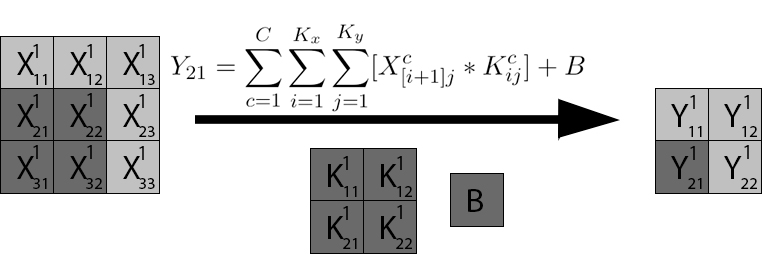
\includegraphics[width=1\linewidth]{imagenes/conv_ejemplo_backprop_3.jpg} 
	\caption{Cálculo de $Y^c_{21}$ mediante propagación hacia delante en una capa convolucional}
	\label{fig:ejemplo_3_forward_prop_convolucional}
\end{figure}

Se calcula el gradiente de $Y^c_{21}$ respecto a cada peso (\ref{grad_y21_k_1} y \ref{grad_y21_k_2})

\begin{gather}
	Y^c_{21} = Z^c_{21} * K^c_{11} + Z^c_{22} * K^c_{12} + Z^c_{31} * K^c_{21} + Z^c_{32} * K^c_{22} \\
	\frac{\partial Y^c_{21}}{\partial K^c_{xy}} = \frac{\partial (Z^c_{21} * K^c_{11} + Z^c_{22} * K^c_{12} + Z^c_{31} * K^c_{21} + Z^c_{32} * K^c_{22})}{\partial K^c_{xy}} \\
	\frac{\partial Y^c_{21}}{\partial K^c_{11}} = Z^c_{21}, \hspace{10mm} \frac{\partial Y^c_{21}}{\partial K^c_{12}} = Z^c_{22} \label{grad_y21_k_1} \\
	\frac{\partial Y^c_{21}}{\partial K^c_{21}} = Z^c_{31}, \hspace{10mm} \frac{\partial Y^c_{21}}{\partial K^c_{22}} = Z^c_{32} \label{grad_y21_k_2}
\end{gather}

 y valor de entrada (\ref{grad_y21_z_1}, \ref{grad_y21_z_2} y \ref{grad_y21_z_3}).
 
\begin{gather}
	\frac{\partial Y^c_{21}}{\partial Z^c_{11}} = 0, \hspace{16mm} \frac{\partial Y^c_{21}}{\partial Z^c_{12}} = 0, \hspace{13mm} \frac{\partial Y^c_{21}}{\partial Z^c_{13}} = 0 \label{grad_y21_z_1} \\
	\frac{\partial Y^c_{21}}{\partial Z^c_{21}} = K^c_{11}, \hspace{10mm} \frac{\partial Y^c_{21}}{\partial Z^c_{22}} = K^c_{12}, \hspace{10mm} \frac{\partial Y^c_{21}}{\partial Z^c_{23}} = 0 \label{grad_y21_z_2} \\
	\frac{\partial Y^c_{21}}{\partial Z^c_{31}} = K^c_{21}, \hspace{10mm} \frac{\partial Y^c_{21}}{\partial Z^c_{32}} = K^c_{22}, \hspace{10mm} \frac{\partial Y^c_{21}}{\partial Z^c_{33}} = 0 \label{grad_y21_z_3}
\end{gather}


\subsubsection{Gradiente de $Y^c_{22}$}

\begin{figure}[H]
	\centering
	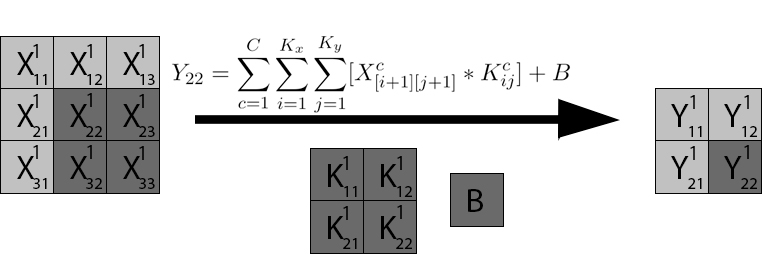
\includegraphics[width=1\linewidth]{imagenes/conv_ejemplo_backprop_4.jpg} 
	\caption{Cálculo de $Y^c_{22}$ mediante propagación hacia delante en una capa convolucional}
	\label{fig:ejemplo_4_forward_prop_convolucional}
\end{figure}

Se calcula el gradiente de $Y^c_{22}$ respecto a cada peso (\ref{grad_y22_k_1}, \ref{grad_y22_k_2}).

\begin{gather}
	Y^c_{22} = Z^c_{22} * K^c_{11} + Z^c_{23} * K^c_{12} + Z^c_{32} * K^c_{21} + Z^c_{33} * K^c_{22} \\
	\frac{\partial Y^c_{22}}{\partial K^c_{xy}} = \frac{\partial (Z^c_{11} * K^c_{11} + Z^c_{12} * K^c_{12} + Z^c_{21} * K^c_{21} + Z^c_{22} * K^c_{22})}{\partial K^c_{xy}} \\
	\frac{\partial Y^c_{22}}{\partial K^c_{11}} = Z^c_{22}, \hspace{10mm} \frac{\partial Y^c_{22}}{\partial K^c_{12}} = Z^c_{23} \label{grad_y22_k_1} \\
	\frac{\partial Y^c_{22}}{\partial K^c_{21}} = Z^c_{32}, \hspace{10mm} \frac{\partial Y^c_{22}}{\partial K^c_{22}} = Z^c_{33} \label{grad_y22_k_2}
\end{gather}

Se calcula el gradiente de $Y^c_{22}$ respecto a cada valor del volumen de entrada (\ref{grad_y22_z_1}, \ref{grad_y22_z_2}, y \ref{grad_y22_z_3}).

\begin{gather}
	\frac{\partial Y^c_{22}}{\partial Z^c_{11}} = 0, \hspace{10mm} \frac{\partial Y^c_{22}}{\partial Z^c_{12}} = 0, \hspace{15mm} \frac{\partial Y^c_{22}}{\partial Z^c_{13}} = 0 \hspace{4mm} \label{grad_y22_z_1} \\
	\frac{\partial Y^c_{22}}{\partial Z^c_{21}} = 0, \hspace{10mm} \frac{\partial Y^c_{22}}{\partial Z^c_{22}} = K^c_{11}, \hspace{10mm} \frac{\partial Y^c_{22}}{\partial Z^c_{23}} = K^c_{12} \label{grad_y22_z_2} \\
	\frac{\partial Y^c_{22}}{\partial Z^c_{31}} = 0, \hspace{10mm} \frac{\partial Y^c_{22}}{\partial Z^c_{32}} = K^c_{21}, \hspace{10mm} \frac{\partial Y^c_{22}}{\partial Z^c_{33}} = K^c_{22} \label{grad_y22_z_3}
\end{gather}

\subsubsection{Gradiente respecto a pesos como convolución}

Finalmente, se calcula la sumatoria total de gradientes respecto a cada peso de la capa (\ref{grad_Y_K_1}, \ref{grad_Y_K_2}, \ref{grad_Y_K_3}, \ref{grad_Y_K_4}) y se observa un claro patrón.

\begin{gather}
	\frac{\partial E}{\partial K^c_{11}} = \frac{\partial E}{\partial Y^c_{11}} * Z^c_{11} + \frac{\partial E}{\partial Y^c_{12}} * Z^c_{12} + \frac{\partial E}{\partial Y^c_{21}} * Z^c_{21} + \frac{\partial E}{\partial Y^c_{22}} * Z^c_{22} \label{grad_Y_K_1} \\
	\frac{\partial E}{\partial K^c_{12}} = \frac{\partial E}{\partial Y^c_{11}} * Z^c_{12} + \frac{\partial E}{\partial Y^c_{12}} * Z^c_{13} + \frac{\partial E}{\partial Y^c_{21}} * Z^c_{22} + \frac{\partial E}{\partial Y^c_{22}} * Z^c_{23} \label{grad_Y_K_2} \\	
	\frac{\partial E}{\partial K^c_{21}} = \frac{\partial E}{\partial Y^c_{11}} * Z^c_{21} + \frac{\partial E}{\partial Y^c_{12}} * Z^c_{22} + \frac{\partial E}{\partial Y^c_{31}} * Z^c_{21} + \frac{\partial E}{\partial Y^c_{22}} * Z^c_{32} \label{grad_Y_K_3} \\
	\frac{\partial E}{\partial K^c_{22}} = \frac{\partial E}{\partial Y^c_{11}} * Z^c_{22} + \frac{\partial E}{\partial Y^c_{12}} * Z^c_{23} + \frac{\partial E}{\partial Y^c_{31}} * Z^c_{32} + \frac{\partial E}{\partial Y^c_{22}} * Z^c_{33} \label{grad_Y_K_4}
\end{gather}

Tal y como se observa en los cálculos obtenidos, estos coinciden con una convolución entre la entrada X y el gradiente respecto a la capa de salida Y. Esto se ve con detalle en la figura \ref{fig:conv_backprop_como_convolucion_X_Y} \cite{conv_backprop}.

\begin{figure}[H]
	\centering
	\begin{subfigure}{.5\textwidth}
		\hspace{-25mm}
		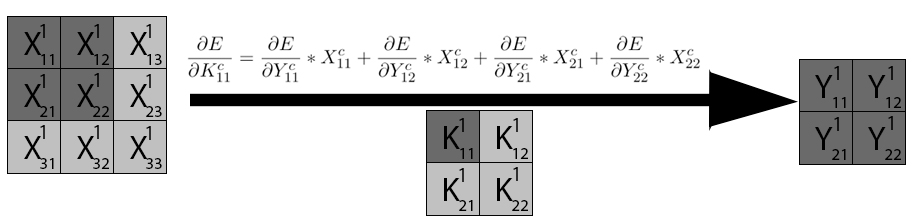
\includegraphics[width=1.4\linewidth]{imagenes/conv_backprop_1.jpg}  
		\caption{Cálculo de $\frac{\partial E}{\partial K^1_{11}}$}
	\end{subfigure}%
	\begin{subfigure}{.5\textwidth}
		\hspace{5mm}
		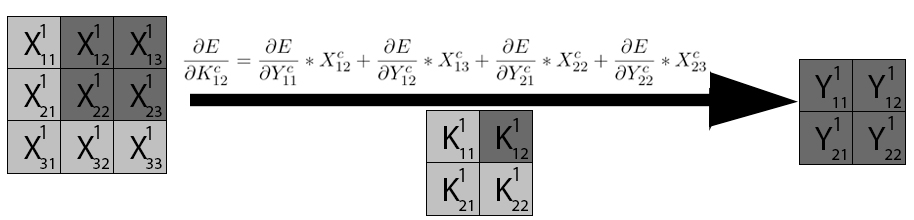
\includegraphics[width=1.4\linewidth]{imagenes/conv_backprop_2.jpg}  
		\caption{Cálculo de $\frac{\partial E}{\partial K^1_{12}}$}
	\end{subfigure}
	\vspace{5mm}
	\begin{subfigure}{.5\textwidth}
	\hspace{-25mm}
	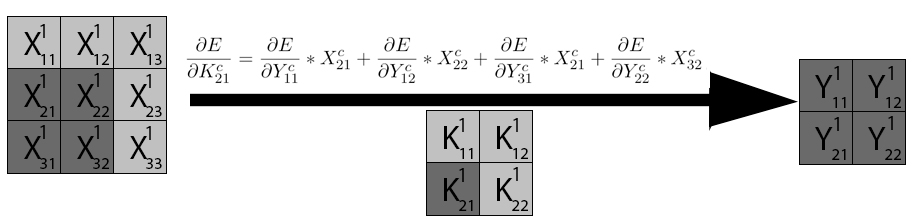
\includegraphics[width=1.4\linewidth]{imagenes/conv_backprop_3.jpg}  
	\caption{Cálculo de $\frac{\partial E}{\partial K^1_{21}}$}
	\end{subfigure}%
	\begin{subfigure}{.5\textwidth}
	\hspace{5mm}
	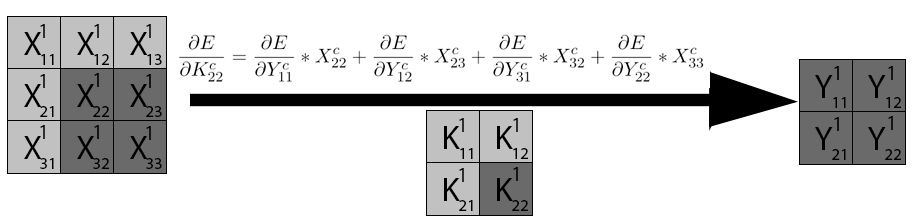
\includegraphics[width=1.4\linewidth]{imagenes/conv_backprop_4.jpg}  
	\caption{Cálculo de $\frac{\partial E}{\partial K^1_{22}}$}
	\end{subfigure}
	\caption{Cálculo del gradiente de la pérdida respecto a cada filtro como convolución entre X e Y}
	\label{fig:conv_backprop_como_convolucion_X_Y}
\end{figure}

En la figura \ref{fig:conv_backprop_como_convolucion_X_Y}, cada subfigura $\{(a), (b), (c), (d)\}$ corresponde al cálculo del gradiente respecto a un peso distinto. Aunque a simple vista parezca algo diferente, los cálculos son exactamente los mismos que los obtenidos anteriormente, solo cambia la visualización de los mismos.

\subsubsection{Gradiente respecto a entrada como convolución}

Por simplicidad y seguir tanto la opinión de expertos como a mi experimentación personal, en capas convolucionales se usará ReLU como función de activación. Por tanto, ya se conoce su derivada pues se calculó previamente (\ref{deriv_relu}).


\begin{gather}
	\frac{\partial E}{\partial A^c_{11}} = \frac{\partial E}{\partial Y^c_{11}} * K^c_{11} *  ReLU'(A^c_{11}) \\
	\frac{\partial E}{\partial A^c_{12}} = (\frac{\partial E}{\partial Y^c_{11}} * K^c_{12} + \frac{\partial E}{\partial Y^c_{12}} * K^c_{11}) * ReLU'(A^c_{12}) \\
	\frac{\partial E}{\partial A^c_{13}} = \frac{\partial E}{\partial Y^c_{12}} * K^c_{12} * ReLU'(A^c_{13}) \\
\end{gather}

\begin{gather}
	\frac{\partial E}{\partial A^c_{21}} = (\frac{\partial E}{\partial Y^c_{11}} * K^c_{21} + \frac{\partial E}{\partial Y^c_{21}} * K^c_{11}) * ReLU'(A^c_{21}) \\
	\frac{\partial E}{\partial A^c_{22}} = (\frac{\partial E}{\partial Y^c_{11}} * K^c_{22} + \frac{\partial E}{\partial Y^c_{12}} * K^c_{21} + \frac{\partial E}{\partial Y^c_{21}} * K^c_{12} + \frac{\partial E}{\partial Y^c_{22}} * K^c_{11}) * ReLU'(A^c_{22}) \\
	\frac{\partial E}{\partial A^c_{23}} = (\frac{\partial E}{\partial Y^c_{12}} * K^c_{22} + \frac{\partial E}{\partial Y^c_{22}} * K^c_{12}) * ReLU'(A^c_{22})\\
\end{gather}

\begin{gather}
	\frac{\partial E}{\partial A^c_{31}} = \frac{\partial E}{\partial Y^c_{21}} * K^c_{21} * ReLU'(A^c_{31})\\
	\frac{\partial E}{\partial A^c_{32}} = (\frac{\partial E}{\partial Y^c_{21}} * K^c_{22} + \frac{\partial E}{\partial Y^c_{22}} * K^c_{21}) * ReLU'(A^c_{32})\\
	\frac{\partial E}{\partial A^c_{33}} = \frac{\partial E}{\partial Y^c_{22}} * K^c_{22} * ReLU'(A^c_{33})
\end{gather}

Tal y como se observa en los cálculos obtenidos, estos coinciden con una convolución tipo completa o ``full'' entre el gradiente respecto a la capa de salida Y y los pesos K invertidos tanto horizontal como verticalmente. El cálculo del gradiente respecto a cada valor $x \in X$ se ve con detalle en la figura \ref{fig:conv_backprop_como_convolucion_Y_W}, mientras que la forma de invertir los pesos se muestra en la figura \ref{fig:flip_W} \cite{conv_backprop}.

\begin{figure}[H]
	\centering
	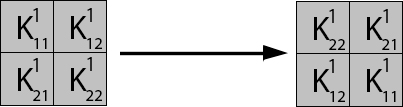
\includegraphics[width=0.8\linewidth]{imagenes/flip_pesos.jpg}  
	\caption{Invertir pesos en K tanto horizontal como verticalmente}
	\label{fig:flip_W}
\end{figure}

\begin{figure}[H]
	\centering
	\begin{subfigure}{.5\textwidth}
		\hspace{-25mm}
		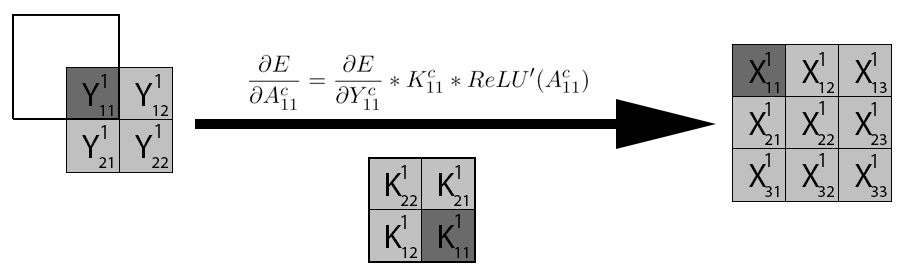
\includegraphics[width=1.4\linewidth]{imagenes/conv_back_entrada_1.jpg}  
		\caption{Gradiente respecto a $X^1_{11}$}
	\end{subfigure}%
	\begin{subfigure}{.5\textwidth}
		\hspace{5mm}
		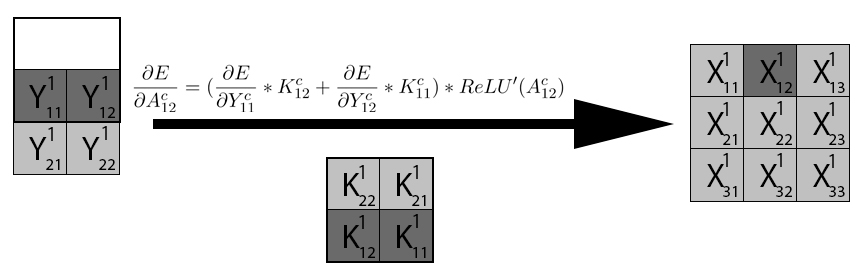
\includegraphics[width=1.4\linewidth]{imagenes/conv_back_entrada_2.jpg}  
		\caption{Gradiente respecto a $X^1_{12}$}
	\end{subfigure}
	\vspace{5mm}
	\begin{subfigure}{.5\textwidth}
		\hspace{-25mm}
		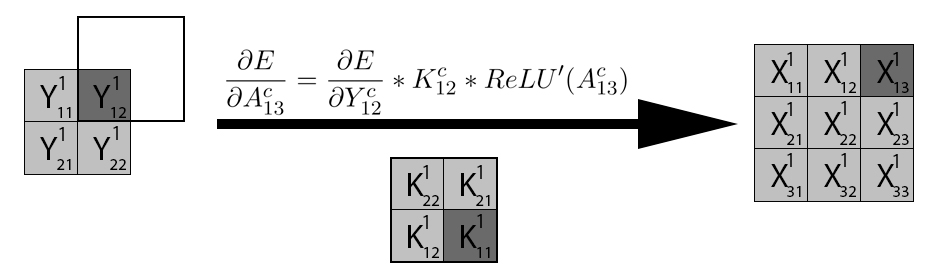
\includegraphics[width=1.4\linewidth]{imagenes/conv_back_entrada_3.jpg}  
		\caption{Gradiente respecto a $X^1_{13}$}
	\end{subfigure}%
	\begin{subfigure}{.5\textwidth}
		\hspace{5mm}
		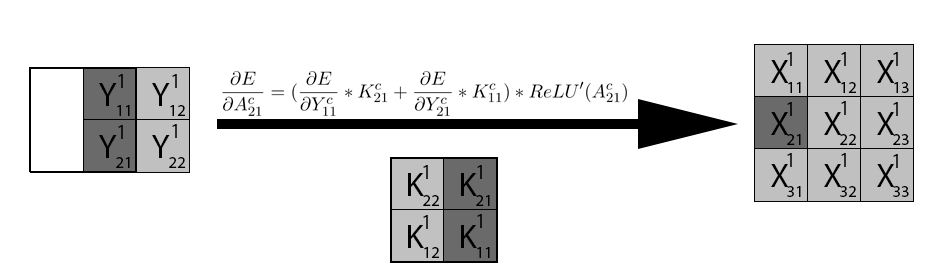
\includegraphics[width=1.4\linewidth]{imagenes/conv_back_entrada_4.jpg}  
		\caption{Gradiente respecto a $X^1_{21}$}
	\end{subfigure}
		\vspace{5mm}
	\begin{subfigure}{.5\textwidth}
		\hspace{-25mm}
		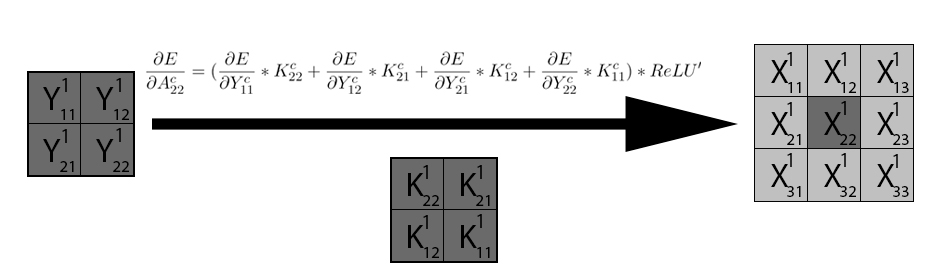
\includegraphics[width=1.4\linewidth]{imagenes/conv_back_entrada_5.jpg}  
		\caption{Gradiente respecto a $X^1_{22}$}
	\end{subfigure}%
	\begin{subfigure}{.5\textwidth}
		\hspace{5mm}
		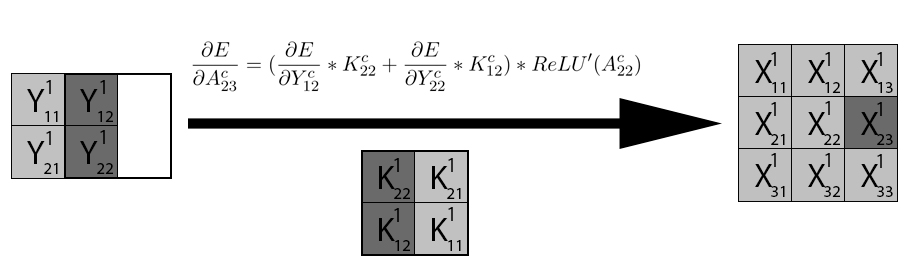
\includegraphics[width=1.4\linewidth]{imagenes/conv_back_entrada_6.jpg}  
		\caption{Gradiente respecto a $X^1_{23}$}
	\end{subfigure}
		\vspace{5mm}
	\begin{subfigure}{.5\textwidth}
		\hspace{-25mm}
		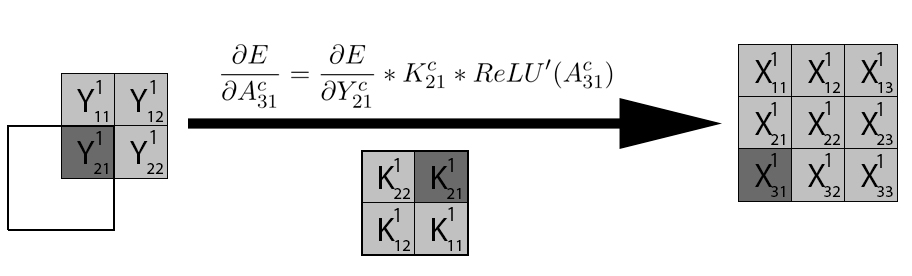
\includegraphics[width=1.4\linewidth]{imagenes/conv_back_entrada_7.jpg}  
		\caption{Gradiente respecto a $X^1_{31}$}
	\end{subfigure}%
	\begin{subfigure}{.5\textwidth}
		\hspace{5mm}
		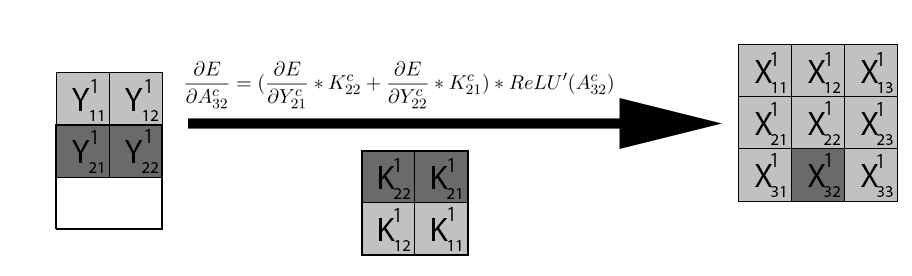
\includegraphics[width=1.4\linewidth]{imagenes/conv_back_entrada_8.jpg}  
		\caption{Gradiente respecto a $X^1_{32}$}
	\end{subfigure}
		\vspace{5mm}
	\begin{subfigure}{.5\textwidth}
		\hspace{-25mm}
		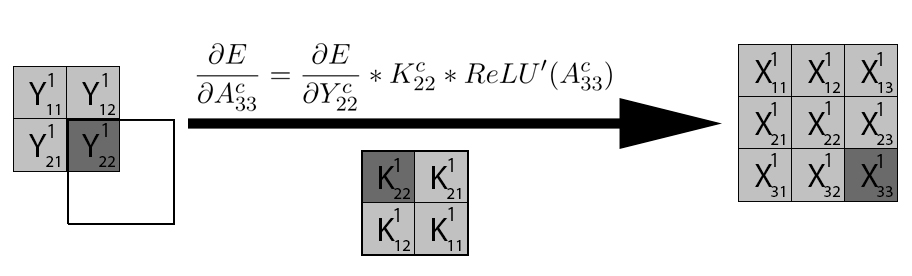
\includegraphics[width=1.4\linewidth]{imagenes/conv_back_entrada_9.jpg}  
		\caption{Gradiente respecto a $X^1_{33}$}
	\end{subfigure}
	\caption{Cálculo del gradiente de la pérdida respecto a cada valor de entrada como convolución entre K e Y}
	\label{fig:conv_backprop_como_convolucion_Y_W}
\end{figure}

Una vez más, los cálculos mostrados en la Figura \ref{fig:conv_backprop_como_convolucion_Y_W} coinciden perfectamente con los obtenidos anteriormente, pues son los mismos. Lo único que cambia es la visualización de los mismos para conseguir una mejor comprensión a escala general y permitir una obtención automática de estos, permitiendo con ello una cómoda implementación en código.

\subsection{Retropropagación con relleno}

\begin{figure}[H]
	\centering
	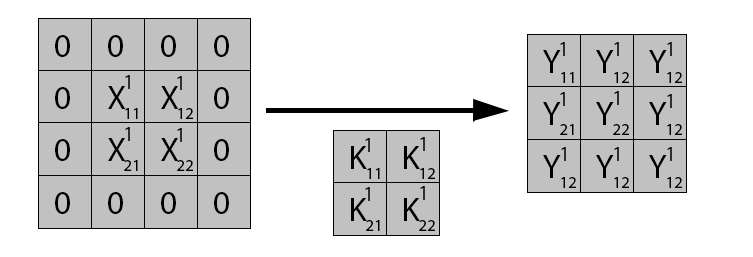
\includegraphics[width=0.8\linewidth]{imagenes/conv_back_padding_intro.jpg} 
	\caption{Ejemplo de retropropagación en una capa convolucional con relleno}
	\label{fig:conv_back_padding_intro}
\end{figure}

Al igual que en el apartado anterior, se realizará y mostrará la retropropagación respecto a una capa convolucional. La principal diferencia en este caso consiste en la presencia de relleno en la capa, tal y como se muestra en el ejemplo a emplear dado por la Figura \ref{fig:conv_back_padding_intro}. Por tanto, a continuación se calculará el gradiente de la función de error respecto a los pesos y los valores de entrada de la capa.

\subsubsection{Gradiente de $Y^c_{11}$}

\begin{figure}[H]
	\centering
	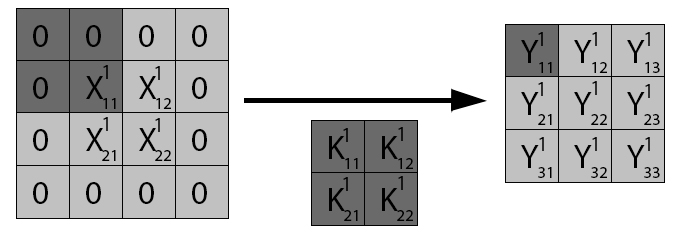
\includegraphics[width=0.8\linewidth]{imagenes/conv_back_padding_1.jpg} 
	\caption{Retropropagación de $Y^c_{11}$}
\end{figure}

Para facilitar la compresión del lector, se mantendrá la misma estructura y notación que en el apartado anterior. \\
Así, se calcula el gradiente de $Y^c_{11}$ respecto a cada peso mediante las fórmulas \ref{gradr_Y11_w_1} y \ref{gradr_Y11_w_1},

\begin{gather}
	Y^c_{11} = Z^c_{11} * K^c_{22} \\
	\frac{\partial Y^c_{11}}{\partial K^c_{xy}} = \frac{\partial (Z^c_{11} * K^c_{22})}{\partial K^c_{xy}} \\
	\frac{\partial Y^c_{11}}{\partial K^c_{11}} = 0, \hspace{10mm} \frac{\partial Y^c_{11}}{\partial K^c_{12}} = 0 \hspace{3mm} \label{gradr_Y11_w_1} \\
	\frac{\partial Y^c_{11}}{\partial K^c_{21}} = 0, \hspace{10mm} \frac{\partial Y^c_{11}}{\partial K^c_{22}} = Z^c_{11} \label{gradr_Y11_w_2}
\end{gather}

así como el gradiente de $Y^c_{11}$ respecto a cada valor del volumen de entrada mediante \ref{gradr_Y11_z_1} y \ref{gradr_Y11_z_2}.

\begin{gather}
	\frac{\partial Y^c_{11}}{\partial Z^c_{11}} = K^c_{22}, \hspace{10mm} \frac{\partial Y^c_{11}}{\partial Z^c_{12}} = 0 \label{gradr_Y11_z_1} \\
	\frac{\partial Y^c_{11}}{\partial Z^c_{21}} = 0, \hspace{14mm} \frac{\partial Y^c_{11}}{\partial Z^c_{22}} = 0 \label{gradr_Y11_z_2}
\end{gather}


\subsubsection{Gradiente de $Y^c_{12}$}

\begin{figure}[H]
	\centering
	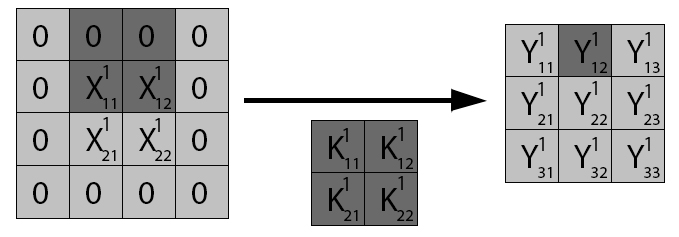
\includegraphics[width=0.8\linewidth]{imagenes/conv_back_padding_2.jpg} 
	\caption{Retropropagación de $Y^c_{12}$}
\end{figure}

Se calcula el gradiente de $Y^c_{12}$ respecto a cada peso mediante \ref{gradr_Y12_w_1} y \ref{gradr_Y12_w_2},

\begin{gather}
	Y^c_{12} = Z^c_{11} * K^c_{21} + Z^c_{12} * K^c_{22} \\
	\frac{\partial Y^c_{12}}{\partial K^c_{xy}} = \frac{\partial (Z^c_{11} * K^c_{21} + Z^c_{12} * K^c_{22})}{\partial K^c_{xy}} \\
	\frac{\partial Y^c_{12}}{\partial K^c_{11}} = 0, \hspace{10mm} \frac{\partial Y^c_{12}}{\partial K^c_{12}} = 0 \label{gradr_Y12_w_1} \\
	\frac{\partial Y^c_{12}}{\partial K^c_{21}} = Z^c_{11}, \hspace{10mm} \frac{\partial Y^c_{12}}{\partial K^c_{22}} = Z^c_{12} \label{gradr_Y12_w_2}
\end{gather}

así como el gradiente de $Y^c_{12}$ respecto a cada valor del volumen de entrada (\ref{gradr_Y12_z_1}, \ref{gradr_Y12_z_2}).

\begin{gather}
	\frac{\partial Y^c_{12}}{\partial Z^c_{11}} = K^c_{21}, \hspace{10mm} \frac{\partial Y^c_{12}}{\partial Z^c_{12}} = K^c_{22} \label{gradr_Y12_z_1} \\
	\frac{\partial Y^c_{12}}{\partial Z^c_{21}} = 0, \hspace{14mm} \frac{\partial Y^c_{12}}{\partial Z^c_{22}} = 0 \hspace{4mm} \label{gradr_Y12_z_2}
\end{gather}

\subsubsection{Gradiente de $Y^c_{13}$}

\begin{figure}[H]
	\centering
	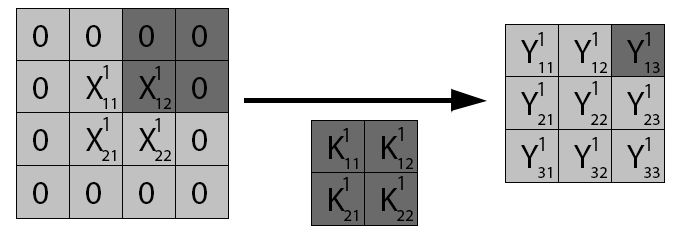
\includegraphics[width=0.8\linewidth]{imagenes/conv_back_padding_3.jpg} 
	\caption{Retropropagación de $Y^c_{13}$}
\end{figure}

Se calcula el gradiente de $Y^c_{13}$ respecto a cada peso mediante \ref{gradr_Y13_w_1} y \ref{gradr_Y13_w_2},

\begin{gather}
	Y^c_{13} = Z^c_{12} * K^c_{21} \\
	\frac{\partial Y^c_{13}}{\partial K^c_{xy}} = \frac{\partial (Z^c_{12} * K^c_{21})}{\partial K^c_{xy}} \\
	\frac{\partial Y^c_{13}}{\partial K^c_{11}} = 0, \hspace{13mm} \frac{\partial Y^c_{13}}{\partial K^c_{12}} = 0 \label{gradr_Y13_w_1} \\
	\frac{\partial Y^c_{13}}{\partial K^c_{21}} = Z^c_{12}, \hspace{10mm} \frac{\partial Y^c_{13}}{\partial K^c_{22}} = 0
\end{gather} \label{gradr_Y13_w_2}

así como el gradiente de $Y^c_{13}$ respecto a cada valor del volumen de entrada (\ref{gradr_Y13_z_1}, \ref{gradr_Y13_z_2}).

\begin{gather}
	\frac{\partial Y^c_{13}}{\partial Z^c_{11}} = 0, \hspace{10mm} \frac{\partial Y^c_{13}}{\partial Z^c_{12}} = K^c_{21} \label{gradr_Y13_z_1} \\
	\frac{\partial Y^c_{13}}{\partial Z^c_{21}} = 0, \hspace{14mm} \frac{\partial Y^c_{13}}{\partial Z^c_{22}} = 0 \hspace{4mm} \label{gradr_Y13_z_2}
\end{gather}


\subsubsection{Gradiente de $Y^c_{21}$}

\begin{figure}[H]
	\centering
	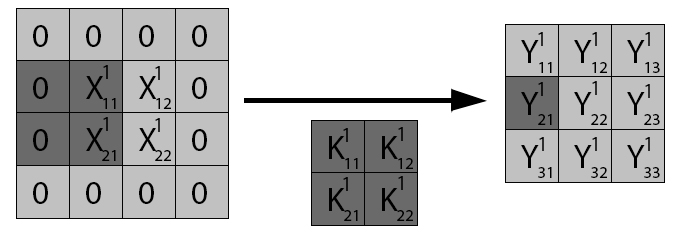
\includegraphics[width=0.8\linewidth]{imagenes/conv_back_padding_4.jpg} 
	\caption{Retropropagación de $Y^c_{21}$}
\end{figure}

Se calcula el gradiente de $Y^c_{21}$ respecto a cada peso mediante \ref{gradr_Y21_w_1} y \ref{gradr_Y21_w_2},


\begin{gather}
	Y^c_{21} = Z^c_{11} * K^c_{12} + Z^c_{21} * K^c_{22} \\
	\frac{\partial Y^c_{21}}{\partial K^c_{xy}} = \frac{\partial (Z^c_{11} * K^c_{12} + Z^c_{21} * K^c_{22})}{\partial K^c_{xy}} \\
	\frac{\partial Y^c_{21}}{\partial K^c_{11}} = 0, \hspace{10mm} \frac{\partial Y^c_{21}}{\partial K^c_{12}} = Z^c_{11} \label{gradr_Y21_w_1} \\
	\frac{\partial Y^c_{21}}{\partial K^c_{21}} = 0, \hspace{10mm} \frac{\partial Y^c_{21}}{\partial K^c_{22}} = Z^c_{21} \label{gradr_Y21_w_2}
\end{gather}

así como el gradiente de $Y^c_{21}$ respecto a cada valor del volumen de entrada (\ref{gradr_Y21_z_1}, \ref{gradr_Y21_z_2}).

\begin{gather}
	\frac{\partial Y^c_{21}}{\partial Z^c_{11}} = K^c_{12}, \hspace{10mm} \frac{\partial Y^c_{21}}{\partial Z^c_{12}} = 0 \label{gradr_Y21_z_1} \\
	\frac{\partial Y^c_{21}}{\partial Z^c_{21}} = K^c_{22}, \hspace{10mm} \frac{\partial Y^c_{21}}{\partial Z^c_{22}} = 0
\end{gather} \label{gradr_Y21_z_2}

\subsubsection{Gradiente de $Y^c_{22}$}

\begin{figure}[H]
	\centering
	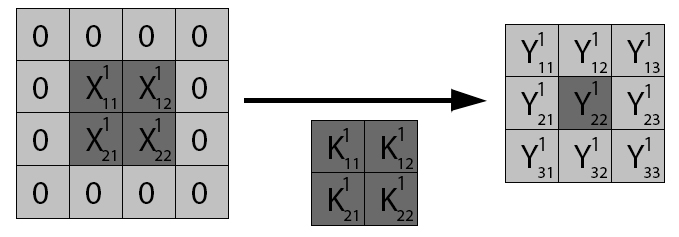
\includegraphics[width=0.8\linewidth]{imagenes/conv_back_padding_5.jpg} 
	\caption{Retropropagación de $Y^c_{22}$}
\end{figure}

Se calcula el gradiente de $Y^c_{22}$ respecto a cada peso mediante \ref{gradr_Y22_w_1} y \ref{gradr_Y22_w_2},


\begin{gather}
	Y^c_{22} = Z^c_{11} * K^c_{11} + Z^c_{12} * K^c_{12} + Z^c_{21} * K^c_{21} + Z^c_{22} * K^c_{22} \\
	\frac{\partial Y^c_{22}}{\partial K^c_{xy}} = \frac{\partial (Z^c_{11} * K^c_{11} + Z^c_{12} * K^c_{12} + Z^c_{21} * K^c_{21} + Z^c_{22} * K^c_{22})}{\partial K^c_{xy}} \\
	\frac{\partial Y^c_{22}}{\partial K^c_{11}} = Z^c_{11}, \hspace{10mm} \frac{\partial Y^c_{22}}{\partial K^c_{12}} = Z^c_{12} \label{gradr_Y22_w_1} \\
	\frac{\partial Y^c_{22}}{\partial K^c_{21}} = Z^c_{21}, \hspace{10mm} \frac{\partial Y^c_{22}}{\partial K^c_{22}} = Z^c_{22} \label{gradr_Y22_w_2}
\end{gather}

así como el gradiente de $Y^c_{22}$ respecto a cada valor del volumen de entrada (\ref{gradr_Y22_z_1}, \ref{gradr_Y22_z_2}).

\begin{gather}
	\frac{\partial Y^c_{22}}{\partial Z^c_{11}} = K^c_{11}, \hspace{10mm} \frac{\partial Y^c_{22}}{\partial Z^c_{12}} = K^c_{12} \label{gradr_Y22_z_1} \\
	\frac{\partial Y^c_{22}}{\partial Z^c_{21}} = K^c_{21}, \hspace{10mm} \frac{\partial Y^c_{22}}{\partial Z^c_{22}} = K^c_{22} \label{gradr_Y22_z_2}.
\end{gather}

\subsubsection{Gradiente de $Y^c_{23}$}

\begin{figure}[H]
	\centering
	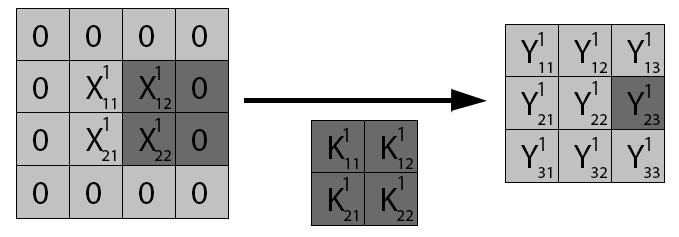
\includegraphics[width=0.8\linewidth]{imagenes/conv_back_padding_6.jpg} 
	\caption{Retropropagación de $Y^c_{23}$}
\end{figure}

Se calcula el gradiente de $Y^c_{23}$ respecto a cada peso mediante \ref{gradr_Y23_w_1} y \ref{gradr_Y23_w_2},


\begin{gather}
	Y^c_{23} = Z^c_{12} * K^c_{11} + Z^c_{22} * K^c_{21} \\
	\frac{\partial Y^c_{23}}{\partial K^c_{xy}} = \frac{\partial (Z^c_{12} * K^c_{11} + Z^c_{22} * K^c_{21})}{\partial K^c_{xy}} \\
	\frac{\partial Y^c_{23}}{\partial K^c_{11}} = Z^c_{12}, \hspace{10mm} \frac{\partial Y^c_{23}}{\partial K^c_{12}} = 0 \label{gradr_Y23_w_1} \\
	\frac{\partial Y^c_{23}}{\partial K^c_{21}} = Z^c_{22}, \hspace{10mm} \frac{\partial Y^c_{23}}{\partial K^c_{22}} = 0 \label{gradr_Y23_w_2}
\end{gather}

así como el gradiente de $Y^c_{23}$ respecto a cada valor del volumen de entrada (\ref{gradr_Y22_z_1}, \ref{gradr_Y22_z_2}).


\begin{gather}
	\frac{\partial Y^c_{23}}{\partial Z^c_{11}} = 0, \hspace{10mm} \frac{\partial Y^c_{23}}{\partial Z^c_{12}} = K^c_{11}\\
	\frac{\partial Y^c_{23}}{\partial Z^c_{21}} = 0, \hspace{10mm} \frac{\partial Y^c_{23}}{\partial Z^c_{22}} = K^c_{21}
\end{gather}

\subsubsection{Gradiente de $Y^c_{31}$}

\begin{figure}[H]
	\centering
	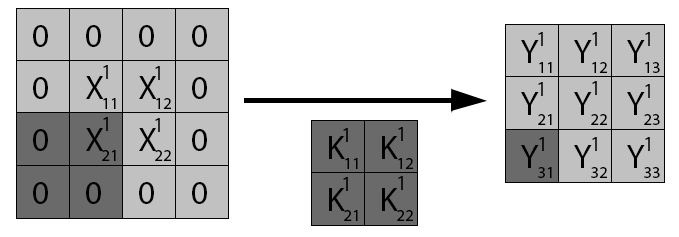
\includegraphics[width=0.8\linewidth]{imagenes/conv_back_padding_7.jpg} 
	\caption{Retropropagación de $Y^c_{31}$}
\end{figure}

Se calcula el gradiente de $Y^c_{31}$ respecto a cada peso mediante \ref{gradr_Y31_w_1} y \ref{gradr_Y31_w_2},

\begin{gather}
	Y^c_{31} = Z^c_{21} * K^c_{12} \\
	\frac{\partial Y^c_{31}}{\partial K^c_{xy}} = \frac{\partial (Z^c_{21} * K^c_{12})}{\partial K^c_{xy}} \\
	\frac{\partial Y^c_{31}}{\partial K^c_{11}} = 0, \hspace{10mm} \frac{\partial Y^c_{31}}{\partial K^c_{12}} = Z^c_{21} \label{gradr_Y31_w_1} \\
	\frac{\partial Y^c_{31}}{\partial K^c_{21}} = 0, \hspace{10mm} \frac{\partial Y^c_{31}}{\partial K^c_{22}} = 0 \hspace{4mm} \label{gradr_Y31_w_2}
\end{gather}

así como el gradiente de $Y^c_{31}$ respecto a cada valor del volumen de entrada (\ref{gradr_Y31_z_1}, \ref{gradr_Y31_z_2}).

\begin{gather}
	\frac{\partial Y^c_{31}}{\partial Z^c_{11}} = 0, \hspace{14mm} \frac{\partial Y^c_{31}}{\partial Z^c_{12}} = 0 \label{gradr_Y31_z_1} \\
	\frac{\partial Y^c_{31}}{\partial Z^c_{21}} = K^c_{12}, \hspace{10mm} \frac{\partial Y^c_{31}}{\partial Z^c_{22}} = 0 \label{gradr_Y31_z_2}
\end{gather}


\subsubsection{Gradiente de $Y^c_{32}$}

\begin{figure}[H]
	\centering
	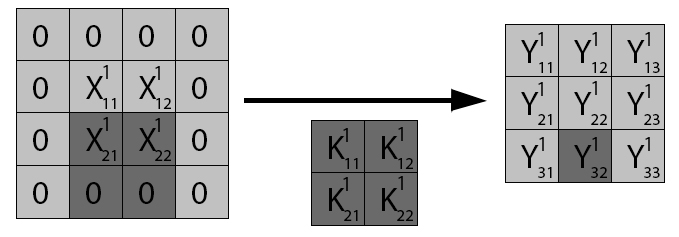
\includegraphics[width=0.8\linewidth]{imagenes/conv_back_padding_8.jpg} 
	\caption{Retropropagación de $Y^c_{32}$}
\end{figure}

Se calcula el gradiente de $Y^c_{32}$ respecto a cada peso mediante \ref{gradr_Y32_w_1} y \ref{gradr_Y32_w_2},

\begin{gather}
	Y^c_{32} = Z^c_{21} * K^c_{11} + Z^c_{22} * K^c_{12} \\
	\frac{\partial Y^c_{32}}{\partial K^c_{xy}} = \frac{\partial (Z^c_{21} * K^c_{11} + Z^c_{22} * K^c_{12})}{\partial K^c_{xy}} \\
	\frac{\partial Y^c_{32}}{\partial K^c_{11}} = Z^c_{21}, \hspace{10mm} \frac{\partial Y^c_{32}}{\partial K^c_{12}} = Z^c_{22} \label{gradr_Y32_w_1} \\
	\frac{\partial Y^c_{32}}{\partial K^c_{21}} = 0, \hspace{14mm} \frac{\partial Y^c_{32}}{\partial K^c_{22}} = 0 \hspace{4mm} \label{gradr_Y32_w_2}
\end{gather}

así como el gradiente de $Y^c_{32}$ respecto a cada valor del volumen de entrada (\ref{gradr_Y32_z_1}, \ref{gradr_Y32_z_2}).


\begin{gather}
	\frac{\partial Y^c_{32}}{\partial Z^c_{11}} = 0, \hspace{14mm} \frac{\partial Y^c_{32}}{\partial Z^c_{12}} = 0 \hspace{4mm} \label{gradr_Y32_z_1} \\
	\frac{\partial Y^c_{32}}{\partial Z^c_{21}} = K^c_{11}, \hspace{10mm} \frac{\partial Y^c_{32}}{\partial Z^c_{22}} = K^c_{12} \label{gradr_Y32_z_2}
\end{gather}



\subsubsection{Gradiente de $Y^c_{33}$}

\begin{figure}[H]
	\centering
	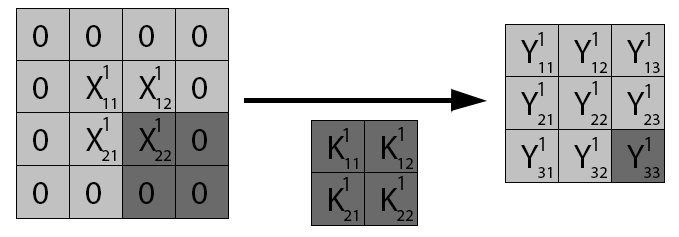
\includegraphics[width=0.8\linewidth]{imagenes/conv_back_padding_9.jpg} 
	\caption{Retropropagación de $Y^c_{33}$}
\end{figure}

Se calcula el gradiente de $Y^c_{33}$ respecto a cada peso mediante \ref{gradr_Y33_w_1} y \ref{gradr_Y33_w_2},


\begin{gather}
	Y^c_{33} = Z^c_{22} * K^c_{11} \\
	\frac{\partial Y^c_{33}}{\partial K^c_{xy}} = \frac{\partial (Z^c_{22} * K^c_{11})}{\partial K^c_{xy}} \\
	\frac{\partial Y^c_{33}}{\partial K^c_{11}} = Z^c_{22}, \hspace{10mm} \frac{\partial Y^c_{33}}{\partial K^c_{12}} = 0 \label{gradr_Y33_w_1} \\
	\frac{\partial Y^c_{33}}{\partial K^c_{21}} = 0, \hspace{14mm} \frac{\partial Y^c_{33}}{\partial K^c_{22}} = 0 \label{gradr_Y33_w_2}
\end{gather}

así como el gradiente de $Y^c_{33}$ respecto a cada valor del volumen de entrada (\ref{gradr_Y33_z_1}, \ref{gradr_Y33_z_2}).


\begin{gather}
	\frac{\partial Y^c_{33}}{\partial Z^c_{11}} = 0, \hspace{10mm} \frac{\partial Y^c_{33}}{\partial Z^c_{12}} = 0 \hspace{4mm} \label{gradr_Y33_z_1} \\
	\frac{\partial Y^c_{33}}{\partial Z^c_{21}} = 0, \hspace{10mm} \frac{\partial Y^c_{33}}{\partial Z^c_{22}} = K^c_{11} \label{gradr_Y33_z_2}
\end{gather}


\subsubsection{Gradiente respecto a pesos como convolución}

Finalmente, al igual que en el caso anterior, se calcula la sumatoria y con ello el gradiente de la función de pérdida respecto a cada peso $K_{xy}$, y una vez más se observa un claro patrón en los resultados obtenidos.

\begin{gather}
	\frac{\partial E}{\partial K^c_{11}} = \frac{\partial E}{\partial Y^c_{22}} * Z^c_{11} + \frac{\partial E}{\partial Y^c_{23}} * Z^c_{12} + \frac{\partial E}{\partial Y^c_{32}} * Z^c_{21} + \frac{\partial E}{\partial Y^c_{33}} * Z^c_{22} \\
	\frac{\partial E}{\partial K^c_{12}} = \frac{\partial E}{\partial Y^c_{21}} * Z^c_{11} + \frac{\partial E}{\partial Y^c_{22}} * Z^c_{12} + \frac{\partial E}{\partial Y^c_{31}} * Z^c_{21} + \frac{\partial E}{\partial Y^c_{32}} * Z^c_{22}\\
	\frac{\partial E}{\partial K^c_{21}} = \frac{\partial E}{\partial Y^c_{12}} * Z^c_{11} + \frac{\partial E}{\partial Y^c_{13}} * Z^c_{12} + \frac{\partial E}{\partial Y^c_{22}} * Z^c_{21} + \frac{\partial E}{\partial Y^c_{23}} * Z^c_{22} \\
	\frac{\partial E}{\partial K^c_{22}} = \frac{\partial E}{\partial Y^c_{11}} * Z^c_{11} + \frac{\partial E}{\partial Y^c_{12}} * Z^c_{12} + \frac{\partial E}{\partial Y^c_{21}} * Z^c_{21} + \frac{\partial E}{\partial Y^c_{22}} * Z^c_{22}
\end{gather}

Tal y como se observa en los cálculos obtenidos, estos coinciden con una convolución entre la entrada X con relleno y el gradiente respecto a la capa de salida Y (figura \ref{fig:conv_backprop_como_convolucion_Xpad_Y}). Como es de esperar, los resultados son exactamente los mismos respecto al caso anterior, salvo que ahora se emplea X con padding en vez de X sin padding para realizar la convolución.

\begin{figure}[H]
	\centering
	\begin{subfigure}{.5\textwidth}
		\hspace{-25mm}
		\includegraphics[width=1.4\linewidth]{imagenes/conv_back_pad_1.jpg}  
		\caption{Cálculo de $\frac{\partial E}{\partial K^1_{11}}$}
	\end{subfigure}%
	\begin{subfigure}{.5\textwidth}
		\hspace{5mm}
		\includegraphics[width=1.4\linewidth]{imagenes/conv_back_pad_2.jpg}  
		\caption{Cálculo de $\frac{\partial E}{\partial K^1_{12}}$}
	\end{subfigure}
	\vspace{5mm}
	\begin{subfigure}{.5\textwidth}
		\hspace{-25mm}
		\includegraphics[width=1.4\linewidth]{imagenes/conv_back_pad_3.jpg}  
		\caption{Cálculo de $\frac{\partial E}{\partial K^1_{21}}$}
	\end{subfigure}%
	\begin{subfigure}{.5\textwidth}
		\hspace{5mm}
		\includegraphics[width=1.4\linewidth]{imagenes/conv_back_pad_4.jpg}  
		\caption{Cálculo de $\frac{\partial E}{\partial K^1_{22}}$}
	\end{subfigure}
	\caption{Cálculo del gradiente de la pérdida respecto a cada filtro como convolución entre X e Y}
	\label{fig:conv_backprop_como_convolucion_Xpad_Y}
\end{figure}

\subsubsection{Gradiente respecto a entrada como convolución}

Una vez más, se empleará ReLU como función de activación en capas convolucionales, tal y como se comentó anteriormente. Por tanto, ya se conoce su derivada pues se calculó previamente (\ref{deriv_relu}).


\begin{gather}
	\frac{\partial E}{\partial A^c_{11}} = (\frac{\partial E}{\partial Y^c_{11}} * K^c_{22} + \frac{\partial E}{\partial Y^c_{12}} * K^c_{21} + \frac{\partial E}{\partial Y^c_{21}} * K^c_{12} + \frac{\partial E}{\partial Y^c_{22}} * K^c_{11}) *  ReLU'(A^c_{11}) \\
	\frac{\partial E}{\partial A^c_{12}} = (\frac{\partial E}{\partial Y^c_{12}} * K^c_{22} + \frac{\partial E}{\partial Y^c_{13}} * K^c_{21} + \frac{\partial E}{\partial Y^c_{22}} * K^c_{12} + \frac{\partial E}{\partial Y^c_{23}} * K^c_{11}) * ReLU'(A^c_{21}) \\
	\frac{\partial E}{\partial A^c_{21}} = (\frac{\partial E}{\partial Y^c_{21}} * K^c_{22} + \frac{\partial E}{\partial Y^c_{22}} * K^c_{21} + \frac{\partial E}{\partial Y^c_{31}} * K^c_{12} + \frac{\partial E}{\partial Y^c_{32}} * K^c_{11}) * ReLU'(A^c_{21}) \\
	\frac{\partial E}{\partial A^c_{22}} = (\frac{\partial E}{\partial Y^c_{22}} * K^c_{22} + \frac{\partial E}{\partial Y^c_{23}} * K^c_{21} + \frac{\partial E}{\partial Y^c_{32}} * K^c_{12} + \frac{\partial E}{\partial Y^c_{33}} * K^c_{11}) * ReLU'(A^c_{22})
\end{gather}

Tal y como se observa en los cálculos obtenidos, estos coinciden con una convolución entre el gradiente respecto a la capa de salida Y y los pesos K invertidos tanto horizontal como verticalmente. Esto se ilustra en detalle en la figura \ref{fig:conv_backprop_como_convolucion_Y_K_pad}.

\begin{figure}[H]
	\centering
	\begin{subfigure}{.5\textwidth}
		\hspace{-25mm}
		\includegraphics[width=1.4\linewidth]{imagenes/conv_back_entrada_pad_1.jpg}  
		\caption{Cálculo de $\frac{\partial E}{\partial A^1_{11}}$}
	\end{subfigure}%
	\begin{subfigure}{.5\textwidth}
		\hspace{5mm}
		\includegraphics[width=1.4\linewidth]{imagenes/conv_back_entrada_pad_2.jpg}  
		\caption{Cálculo de $\frac{\partial E}{\partial A^1_{12}}$}
	\end{subfigure}
	\vspace{5mm}
	\begin{subfigure}{.5\textwidth}
		\hspace{-25mm}
		\includegraphics[width=1.4\linewidth]{imagenes/conv_back_entrada_pad_3.jpg}  
		\caption{Cálculo de $\frac{\partial E}{\partial A^1_{21}}$}
	\end{subfigure}%
	\begin{subfigure}{.5\textwidth}
		\hspace{5mm}
		\includegraphics[width=1.4\linewidth]{imagenes/conv_back_entrada_pad_4.jpg}  
		\caption{Cálculo de $\frac{\partial E}{\partial A^1_{22}}$}
	\end{subfigure}
	\caption{Cálculo del gradiente de la pérdida respecto de la entrada como convolución}
	\label{fig:conv_backprop_como_convolucion_Y_K_pad}
\end{figure}

Una vez desarrolladas ambas retropropagaciones en una capa convolucional (con y sin relleno), se pueden comparar las figuras \ref{fig:conv_backprop_como_convolucion_Y_W} y \ref{fig:conv_backprop_como_convolucion_Y_K_pad} y ver que, aunque ambas calculan el gradiente de la pérdida respecto al volumen de entrada, en una figura se emplea una convolución completa mientras que en la otra no.


\begin{figure}[H]
	\centering
	\begin{subfigure}{.5\textwidth}
		\includegraphics[width=1.4\linewidth]{imagenes/full_vs_normal_conv_1.jpg}  
		\caption{Retropropagación con un nivel de relleno}
	\end{subfigure}
	
	\vspace{5mm}
	\begin{subfigure}{.5\textwidth}
		\includegraphics[width=1.4\linewidth]{imagenes/full_vs_normal_conv_2.jpg}  
		\caption{Retropropagación con dos niveles de relleno}
	\end{subfigure}
	\caption{Cálculo del gradiente de la pérdida respecto a la entrada X con uno o dos niveles de relleno}
	\label{fig:conv_full_vs_normal}
\end{figure}

El motivo de ello se presenta en detalle en la figura \ref{fig:conv_full_vs_normal}. Al realizar una convolución total, se empiezan a calcular los gradientes comenzando por la esquina superior izquierda de X. Sin embargo, sabiendo que X tiene relleno, no es necesario realizar el cálculo de los gradientes respecto a las posiciones de `relleno' de la entrada pues no se emplean en ningún cálculo posterior.
